\begin{figure}[h!]
\centering
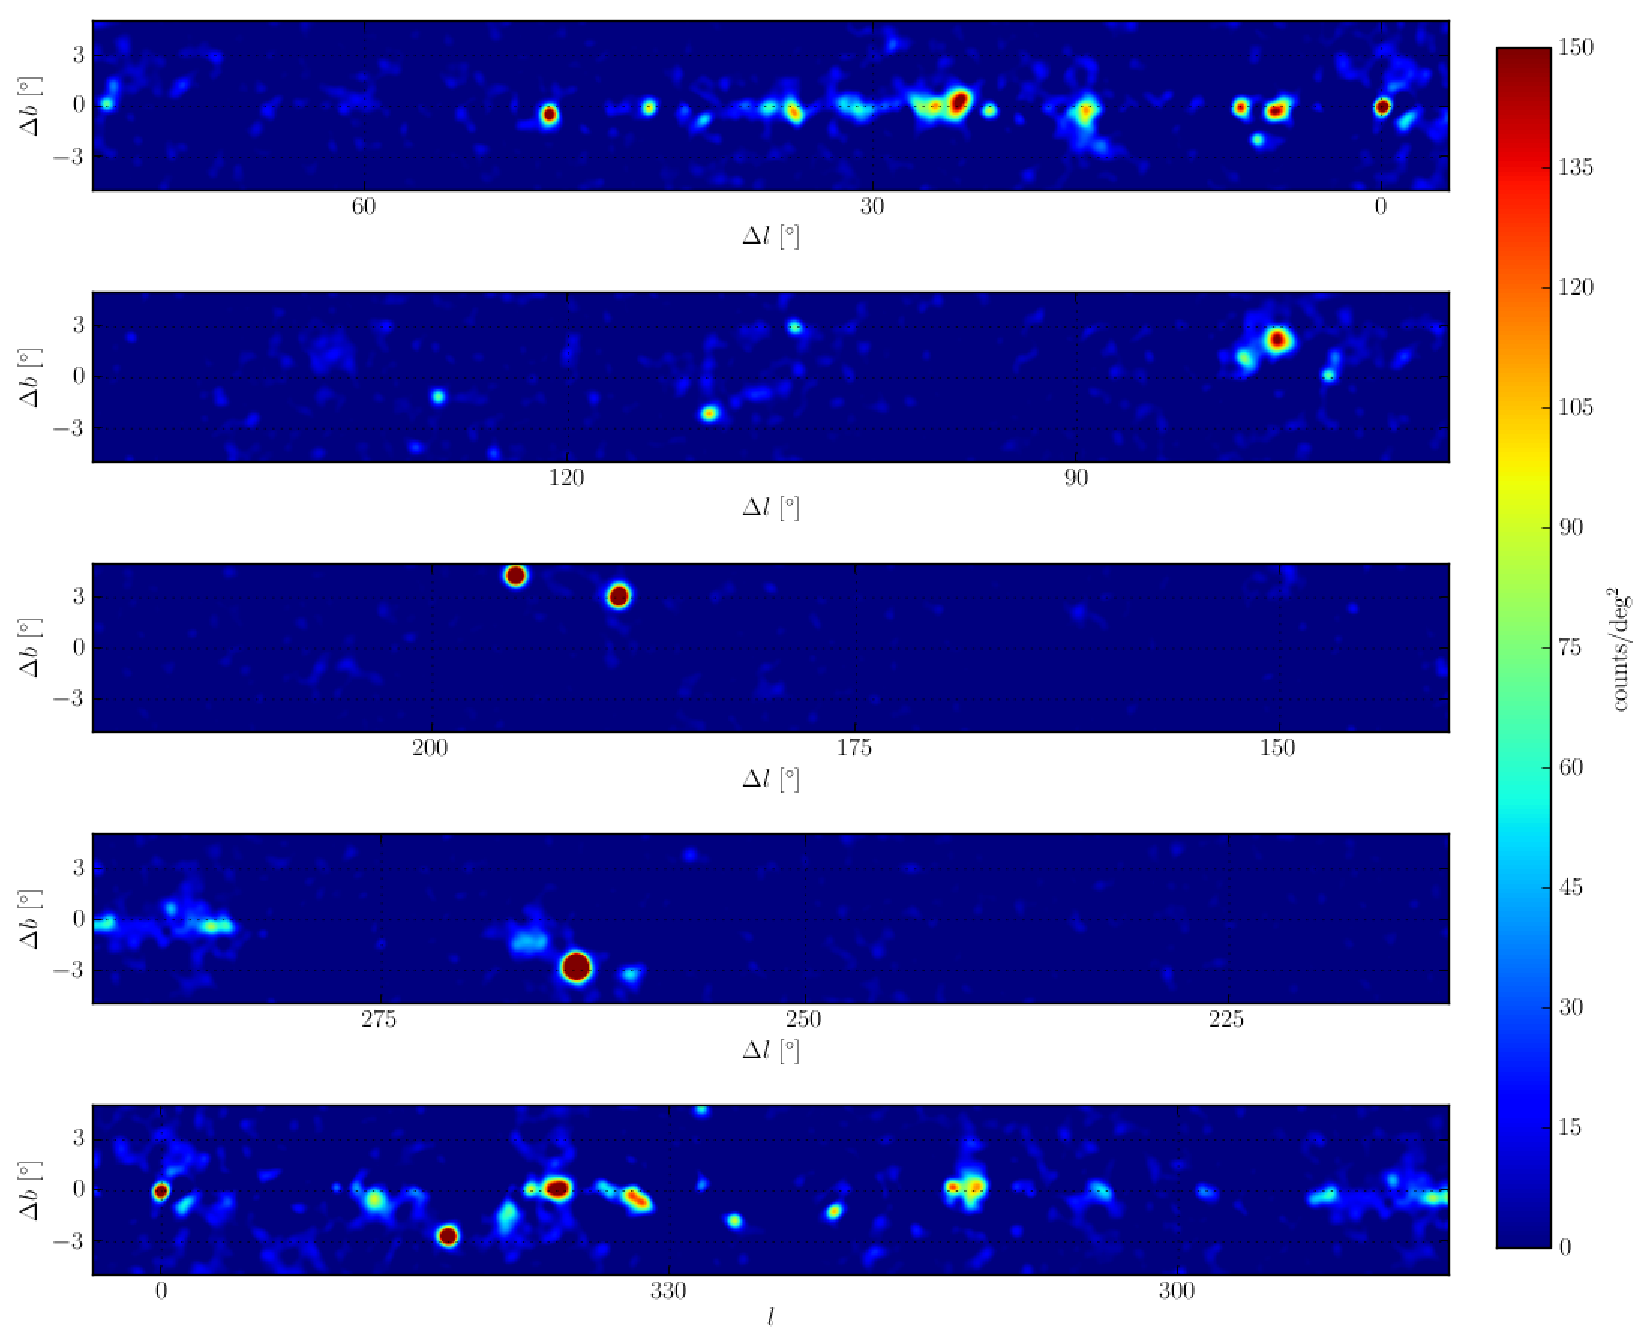
\includegraphics[width=\textwidth]{figures/Plan_gal.eps}
\caption{Residual counts map of the Galactic Plane above 10 GeV. The Galactic and isotropic diffuse emission are subtracted using the files described in section 4.2 with a normalization of 1. All sources associated to Blazars are subtracted using the spectral parameters listed in the hard source list \citep{1FHL}. Excesses visible in this map are due either to Galactic sources or to Blazars not yet associated, emitting above 10 GeV observed by the LAT. The counts map is smoothed with a Gaussian of 0.27$\degr$.
\label{fig:PlanGal}}
\end{figure}

\begin{figure}[h!]
\centering
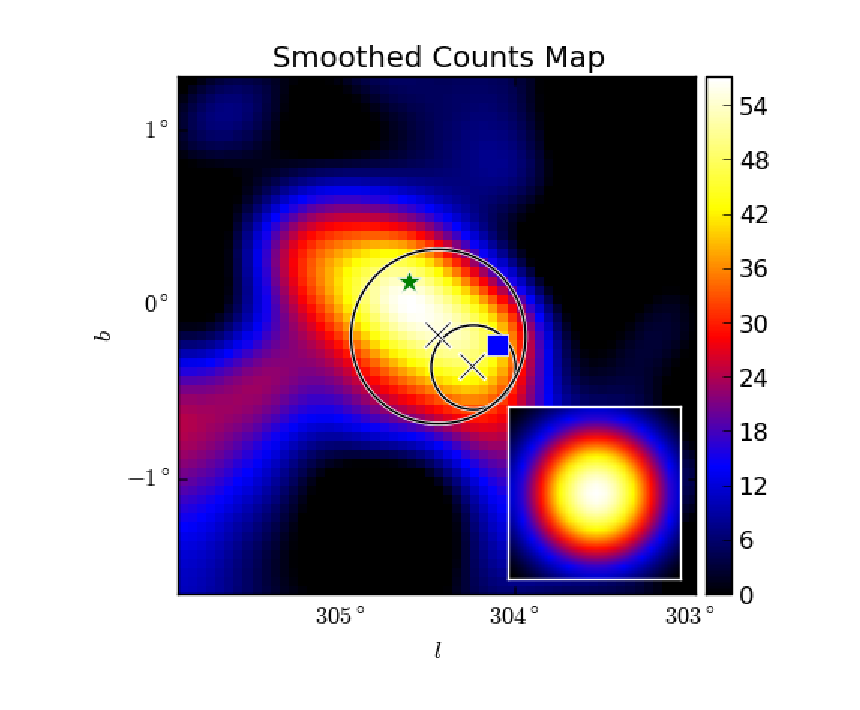
\includegraphics[]{figures/HESSJ1303m631.eps}
\caption{Counts map of the region of HESS~J1303--631. We subtracted the Galactic and isotropic diffuse emission. The counts map is smoothed by a Gaussian of 0.27$\degr$ corresponding to the PSF above 10 GeV. The green star indicates the position of the SNR Kes 17, the blue square represents the position of PSR~J1301--6305. The small and big circles respectively show the extension of the TeV Gaussian proposed by \cite{2005AA...439.1013A} and the extension of the disk derived in this work.
\label{1303}}
\end{figure}

\begin{figure}[h!]
\centering
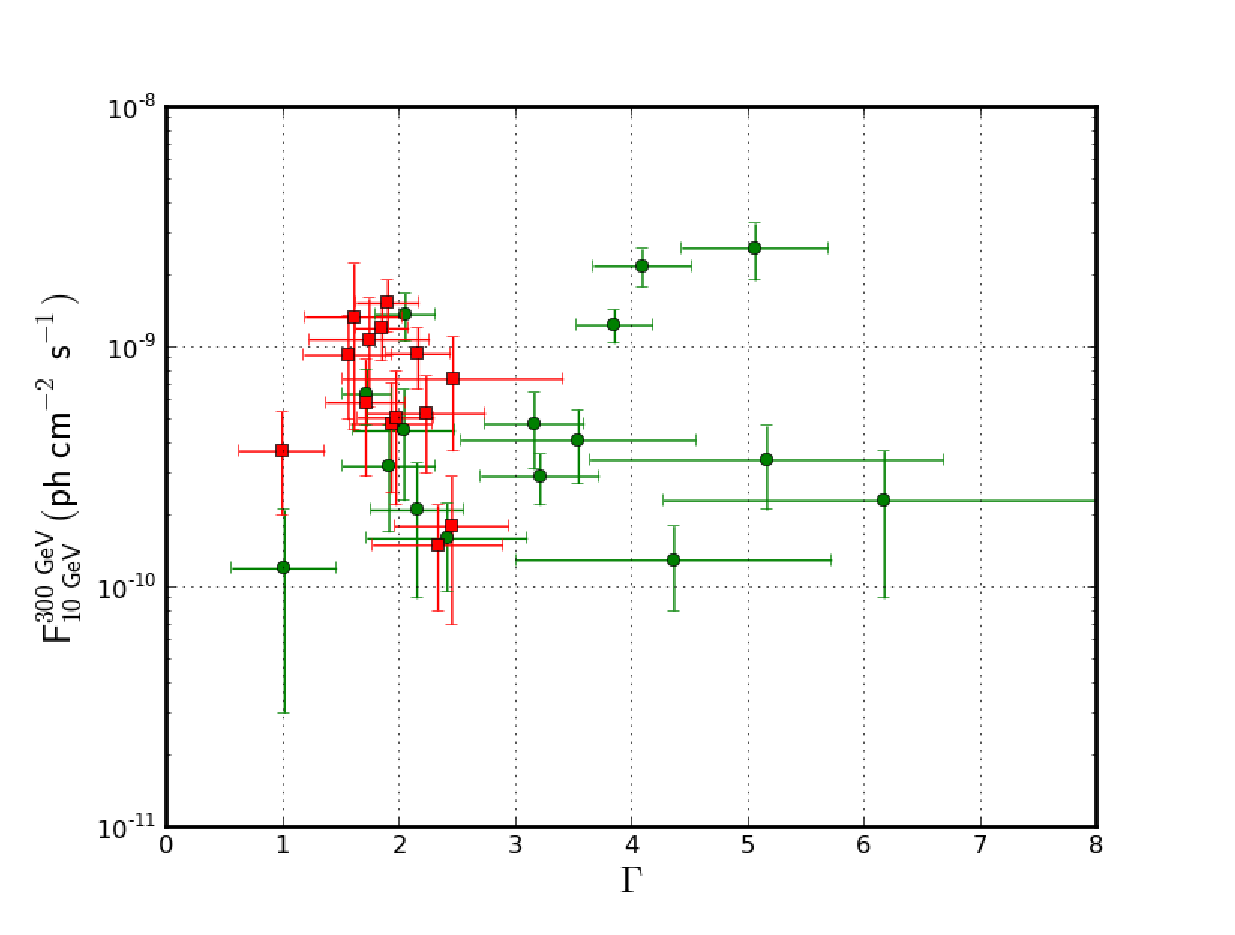
\includegraphics[width=\textwidth]{figures/out_errorbar_best_fit.eps}
\caption{Integrated flux of the detected sources as a function of the power-law index between 10 and 316 GeV (see Table \ref{tab:det_sources}). The green circles show the sources within 0.5$\degr$ of a pulsar detected by the LAT while the red squares represent the sources with no pulsar detected in the GeV energy range within 0.5$\degr$. The error bars show the statistical and systematic uncertainties added in quadrature.  
\label{fig:fluxvssize}}
\end{figure}

\begin{figure}[h!]
\centering
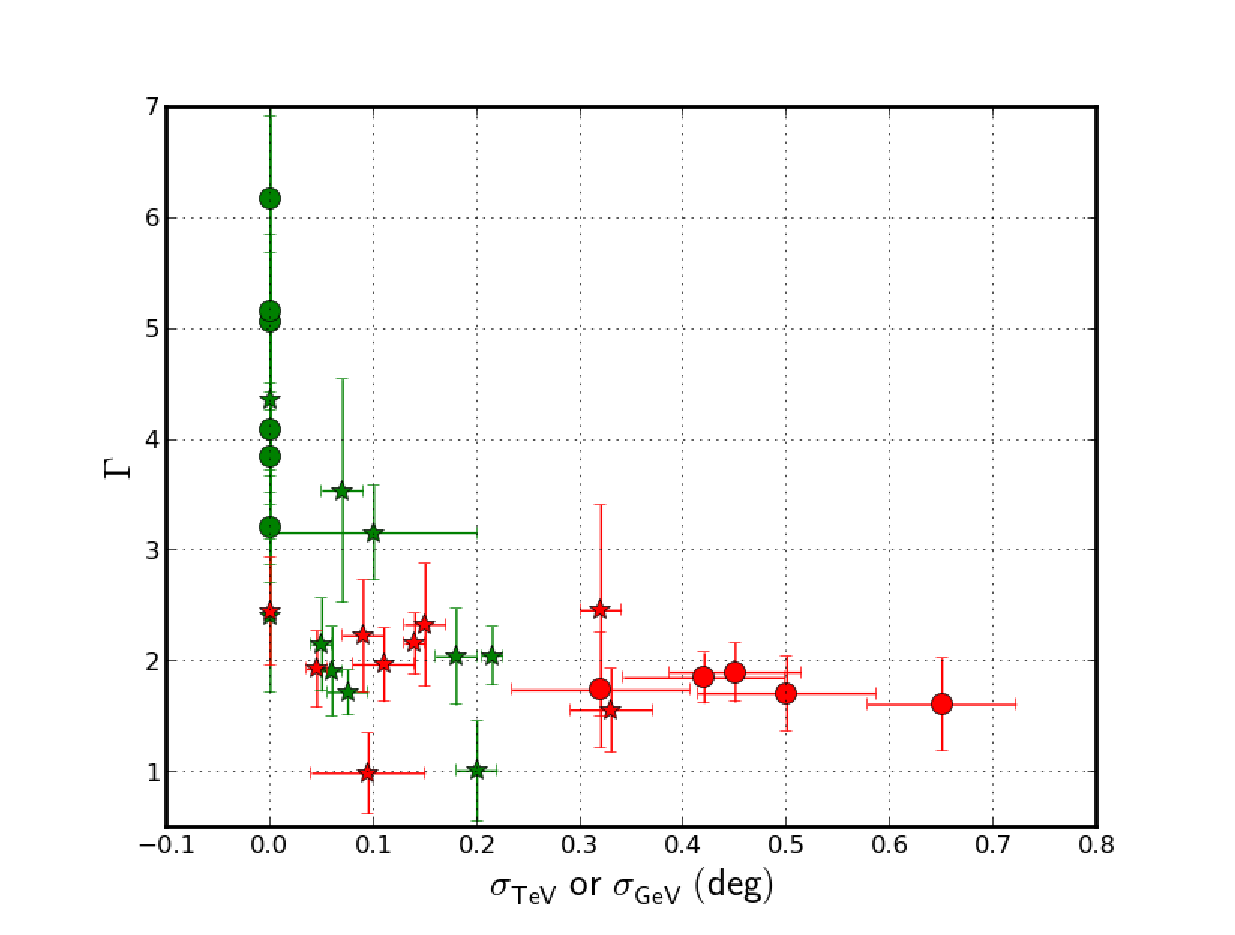
\includegraphics[width=\textwidth]{figures/index_vs_size.eps}
\caption{Spectral index as a function of the GeV or TeV extension for each detected source. The GeV morphology is obtained by fitting the position and extension of the sources as explained in Section \ref{spatanalysis} \& \ref{signi}. The green markers show the sources within 0.5$\degr$ of a pulsar detected by the LAT while the red markers represent the sources with no pulsar detected in the GeV energy range within 0.5$\degr$. The error bars show the statistical and systematic uncertainties added in quadrature. The 11 circles represent the sources for which the GeV morphology significantly improved the fit compared to the TeV morphology (Table \ref{tab:GeVmorph}), while the stars represent the sources modeled assuming their TeV morphology. For sources modelled assuming their TeV morphology, we reported the uncertainties found in the associated reference in Table \ref{tab:TeV_sources}. For asymmetric sources we represented the mean extension with an error bar corresponding to the maximum uncertainty.
\label{fig:indexvssize}}
\end{figure}

%\begin{figure}[h!]
%\centering
%\includegraphics[width=0.5\textwidth]{figures/0FGLJ1958.12848.eps}
%\caption{SED of MGRO J1958$+$2848. The red and blue points show respectively the \emph{Fermi}-LAT and ... points. The black error bars show the statistical and   systematic uncertainties added in quadrature. The black line corresponds to the best fit obtained using the LAT data. The dashed line correspond to the model of PSR J... taken from \cite{2012ApJS..199...31N}.
%\label{fig:1}}
%\end{figure}


\begin{figure}[h!]
\centering
\subfigure{
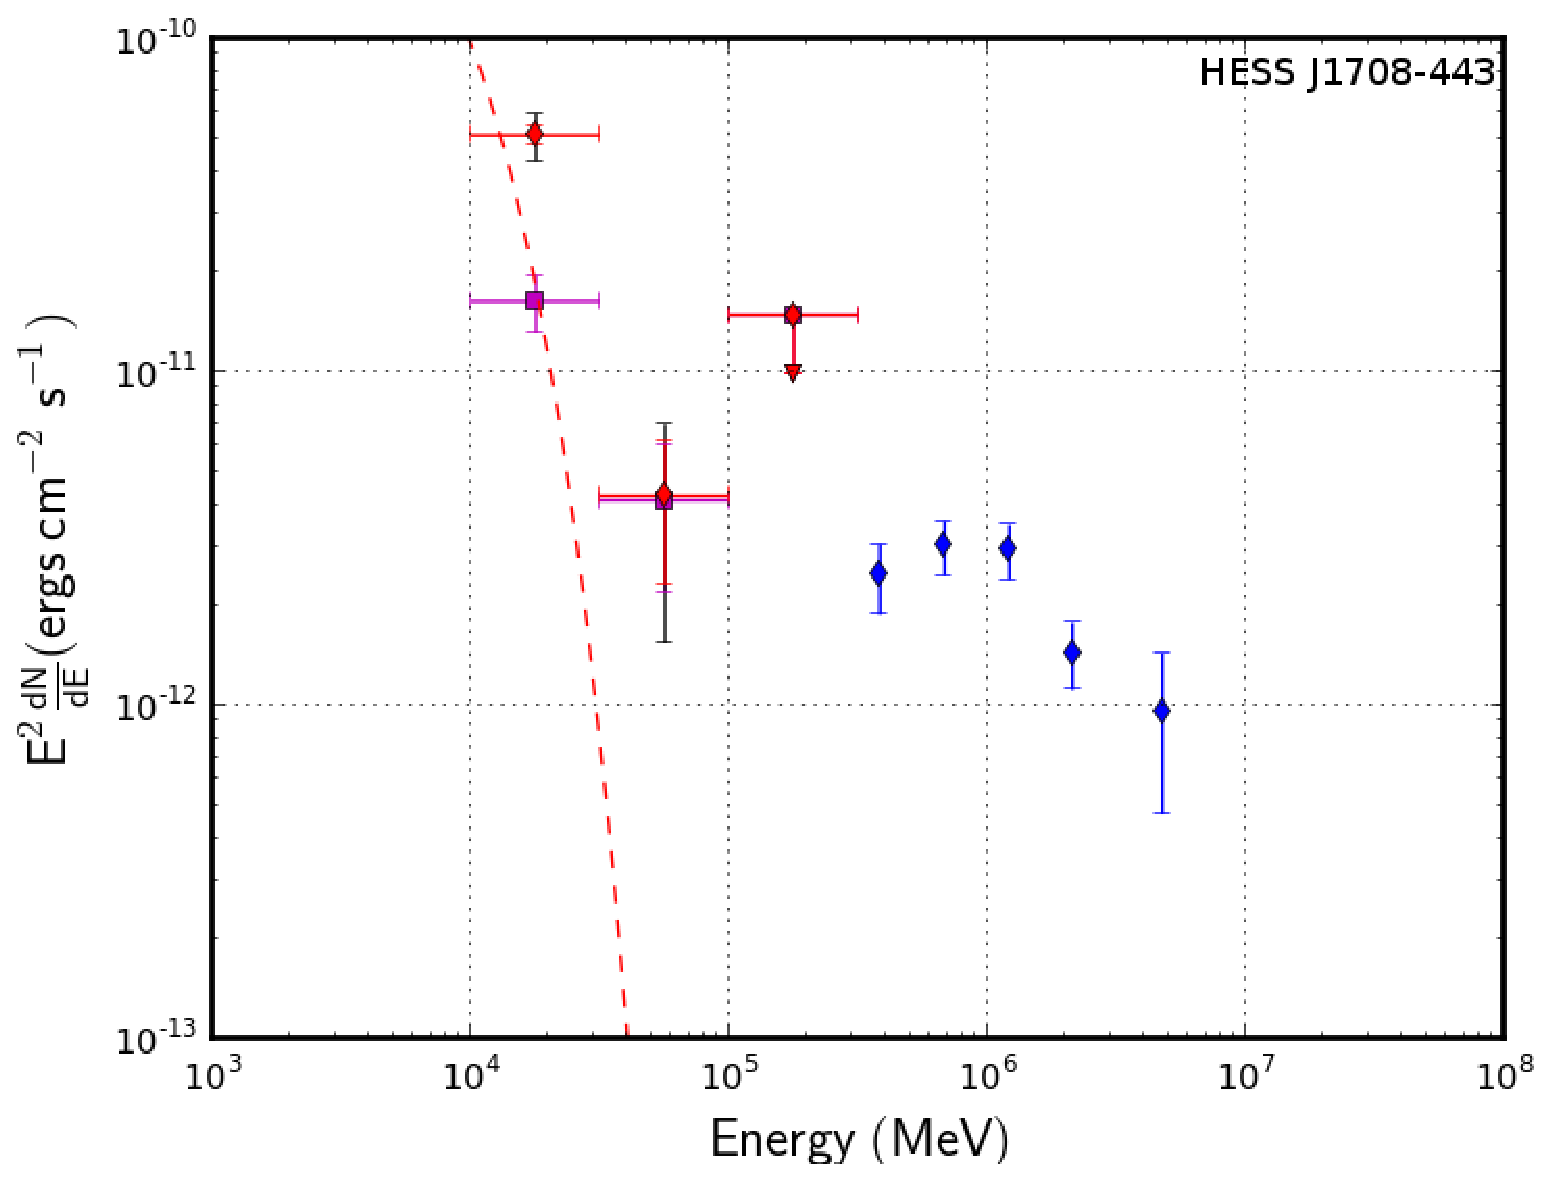
\includegraphics[width=0.45\textwidth]{figures/HESSJ1708.eps}
\label{fig:hess1708}
}
\subfigure{
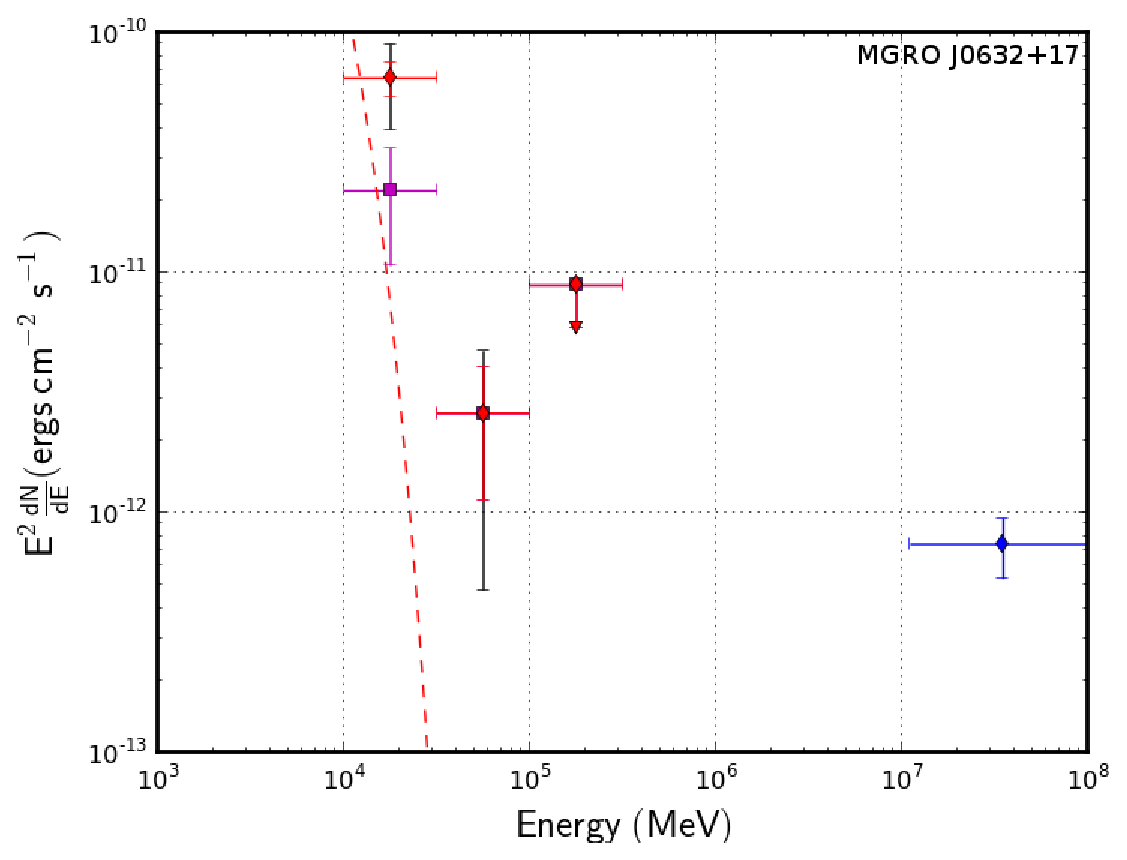
\includegraphics[width=0.45\textwidth]{figures/MGROJ0632.eps}
\label{fig:mgroj0632}
}
\subfigure{
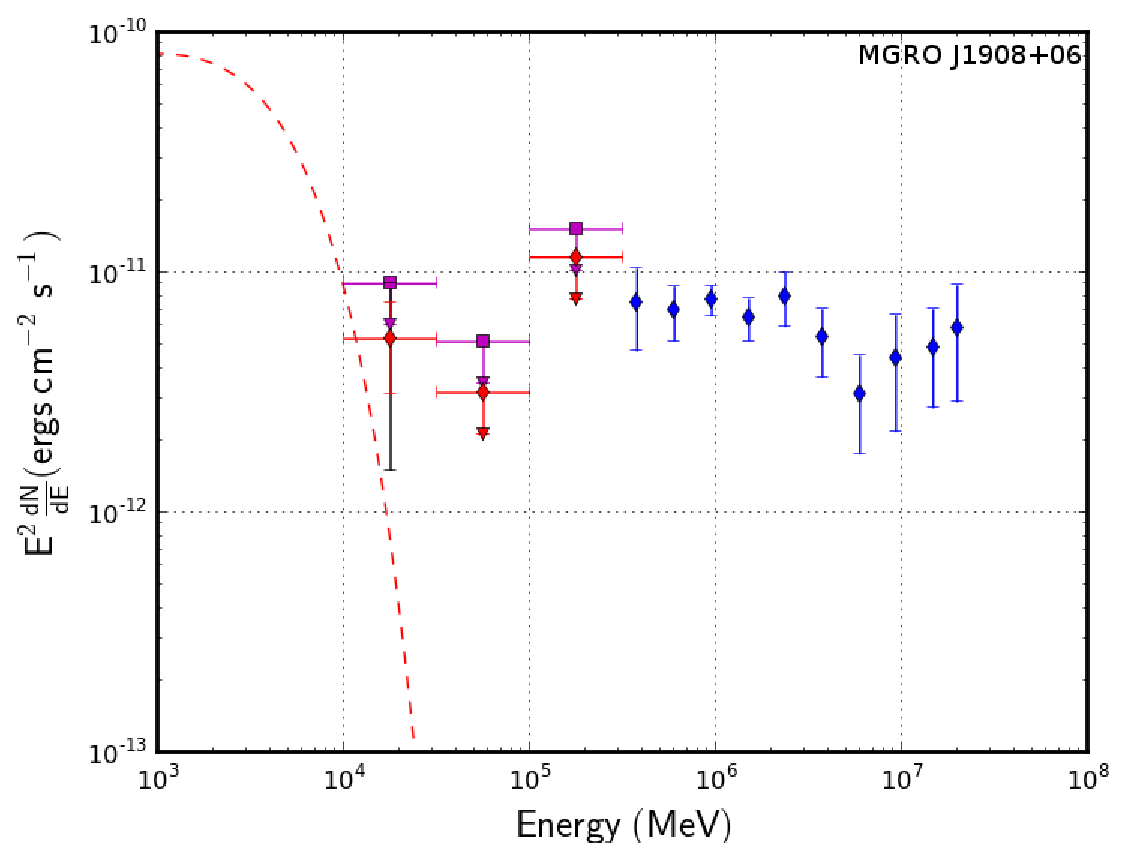
\includegraphics[width=0.45\textwidth]{figures/MGROJ1908.eps}
\label{fig:mgro1908}
}
\subfigure{
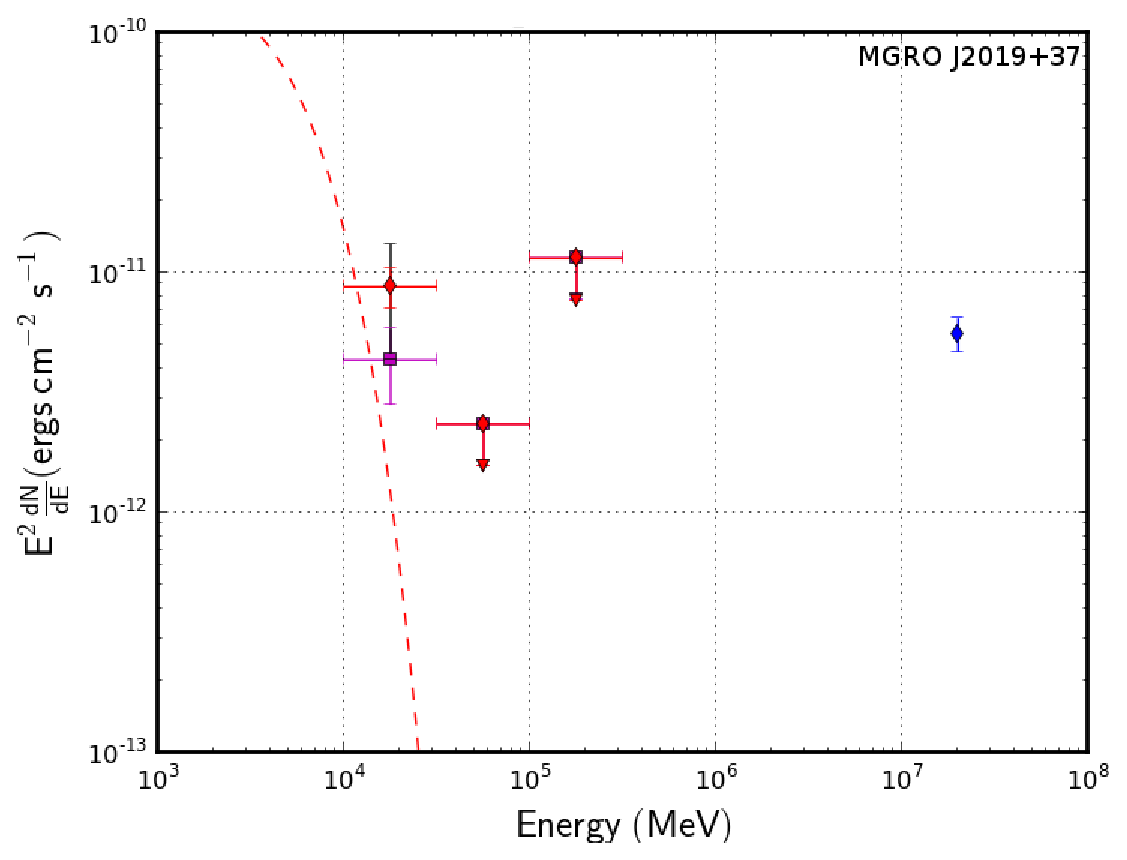
\includegraphics[width=0.45\textwidth]{figures/MGROJ201937.eps}
\label{fig:mgro2019}
}
\subfigure{
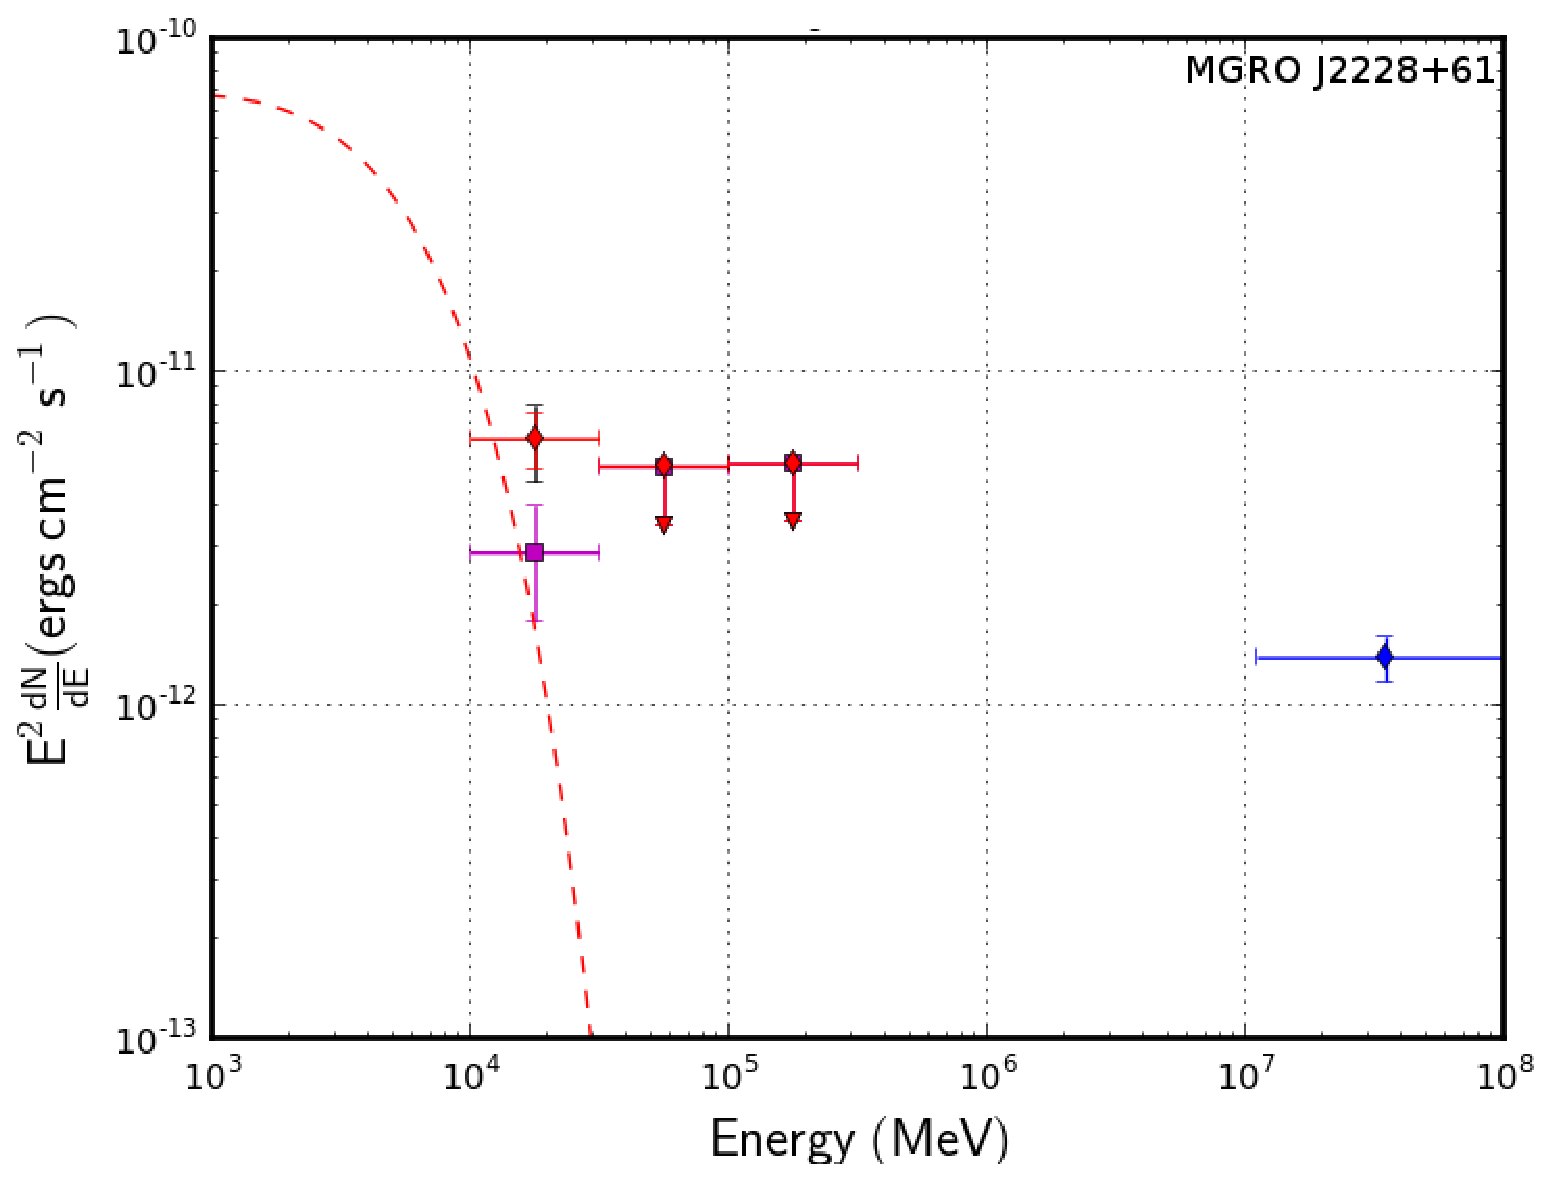
\includegraphics[width=0.45\textwidth]{figures/MGROJ2228.eps}
\label{fig:mgroj2228}
}
\subfigure{
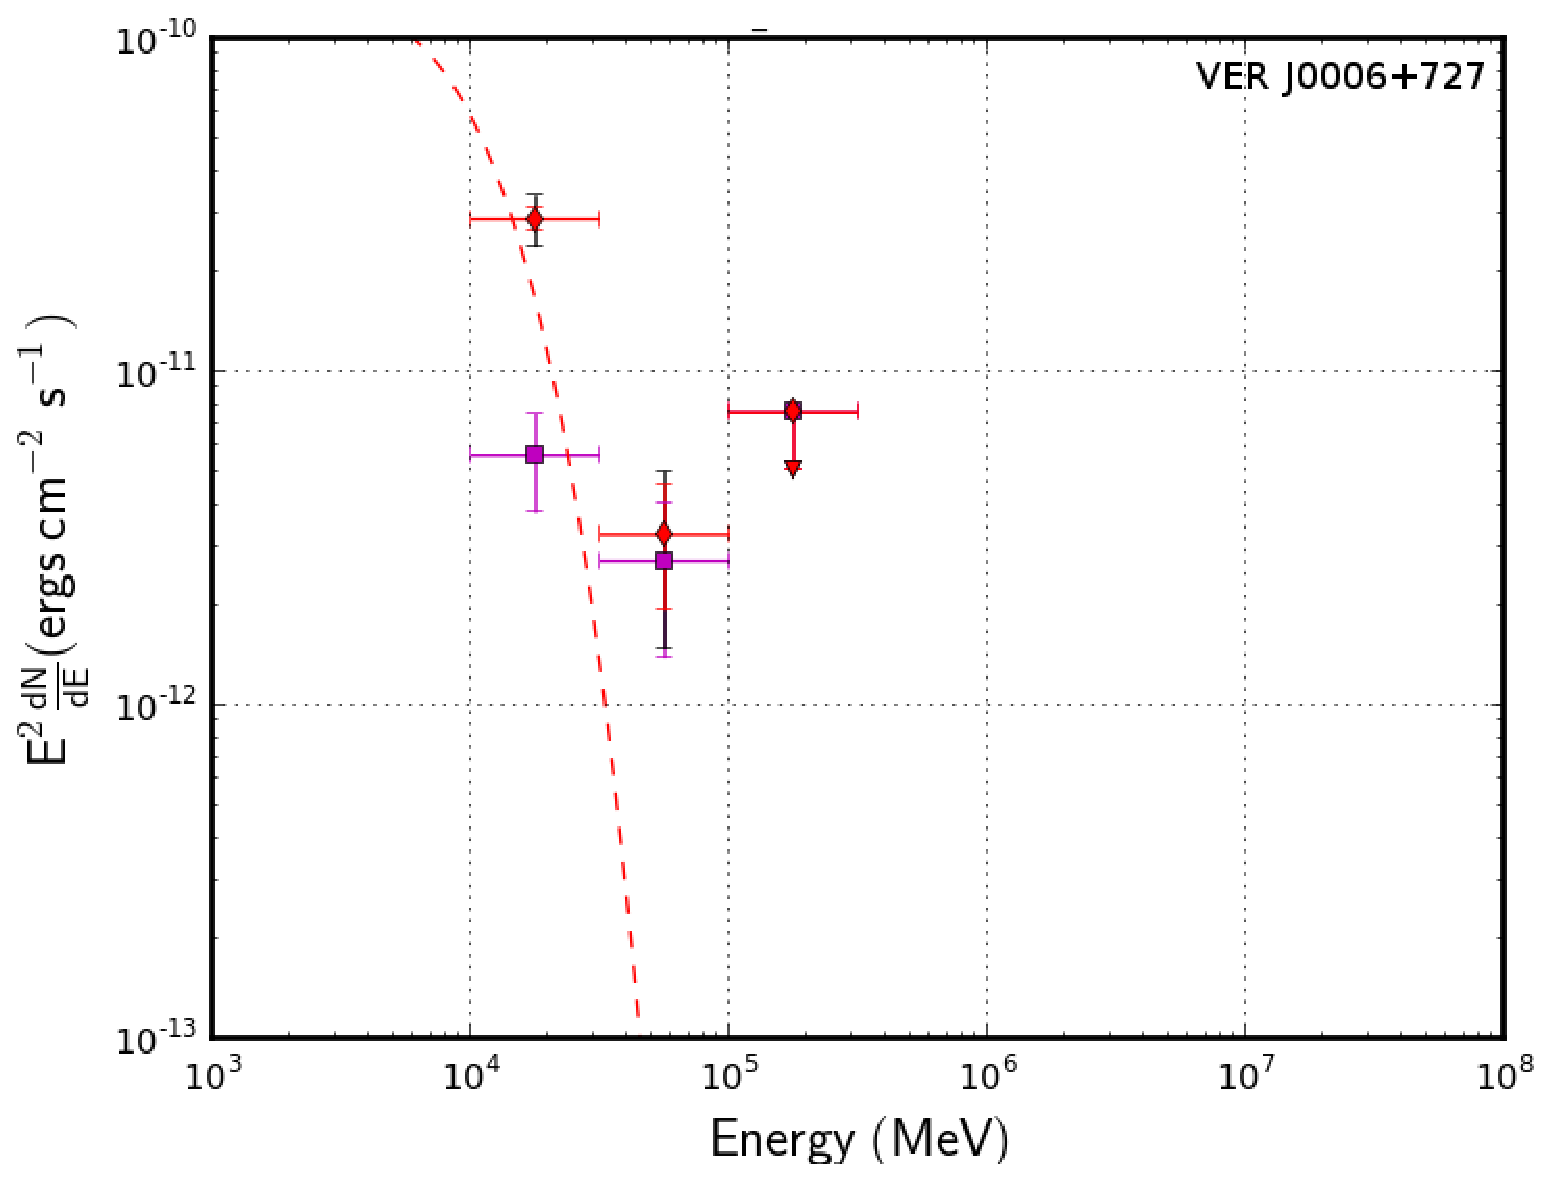
\includegraphics[width=0.45\textwidth]{figures/VERJ0006.eps}
\label{fig:verj0006}
}
\caption{\label{fig:sedsourcespuls}SED of sources better described by a point-like source and with a pulsar within 0.5$\degr$. The blue points show the TeV points taken from \cite{2011AA...528A.143H, 2009ApJ...700L.127A, 2009AA...499..723A, 2007ApJ...664L..91A, 2009ApJ...700L.127A, 2011arXiv1111.2591M}. The red circles and the magenta squares show respectively the SED without the pulsar included in the model and with the pulsar included in the model. The black error bars show the statistical and   systematic uncertainties added in quadrature. The dashed line corresponds to the model of the associated pulsars sumarized in Table \ref{tab:pulsarfit}. In the case of MGRO J1908+06, the red SED was derived assuming a point-like source as determined in Table \ref{tab:GeVmorph} while the magenta SED was derived assuming the TeV shape since it is not significant anymore when the pulsar is included in the model.}
\end{figure}

\begin{figure}[h!]
\centering
\subfigure{
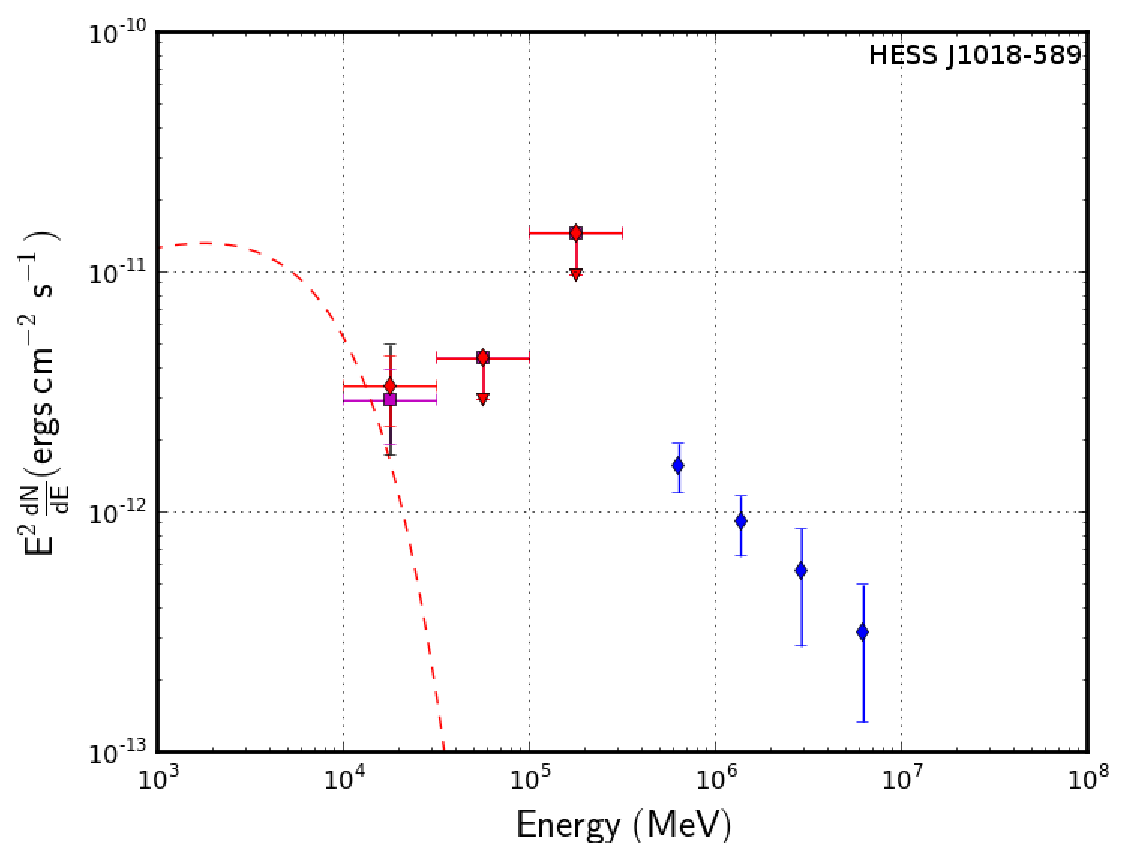
\includegraphics[width=0.45\textwidth]{figures/HESSJ1018.eps}
\label{fig:hessj1018}
}
\subfigure{
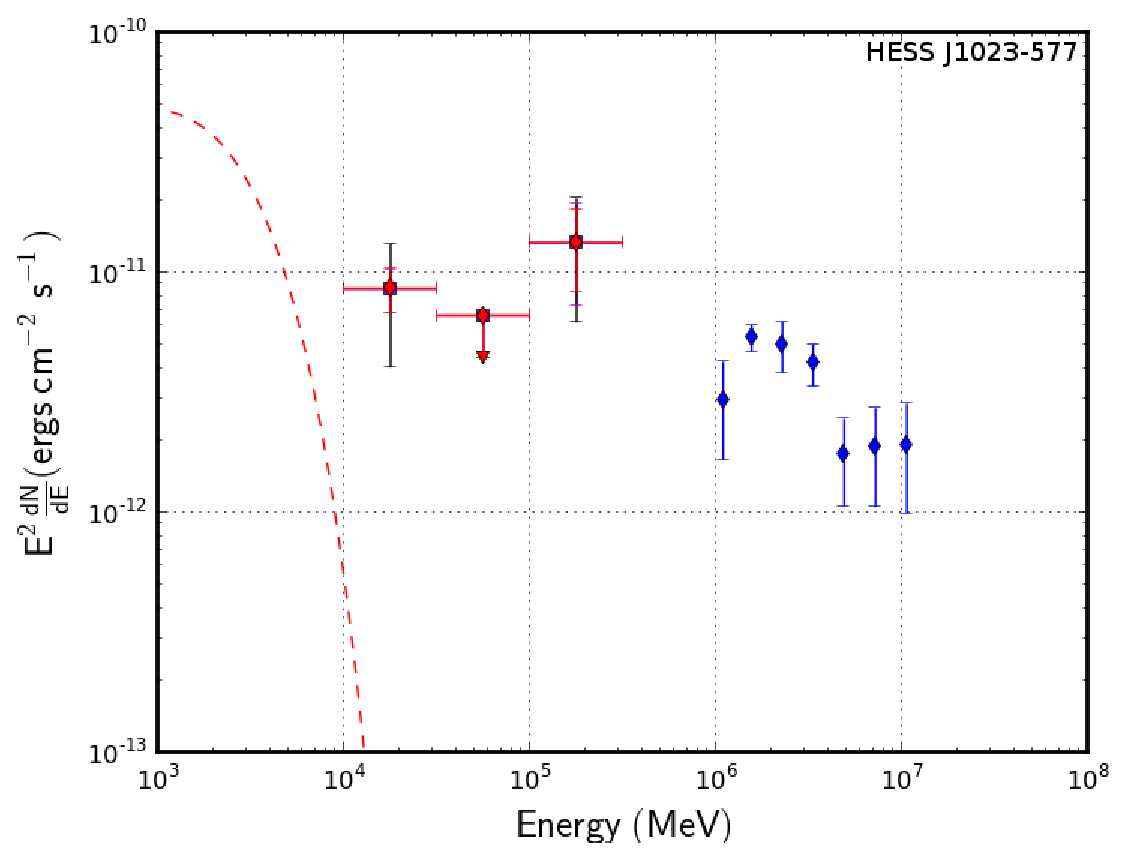
\includegraphics[width=0.45\textwidth]{figures/HESSJ1023.eps}
\label{fig:hessj1023}
}
\subfigure{
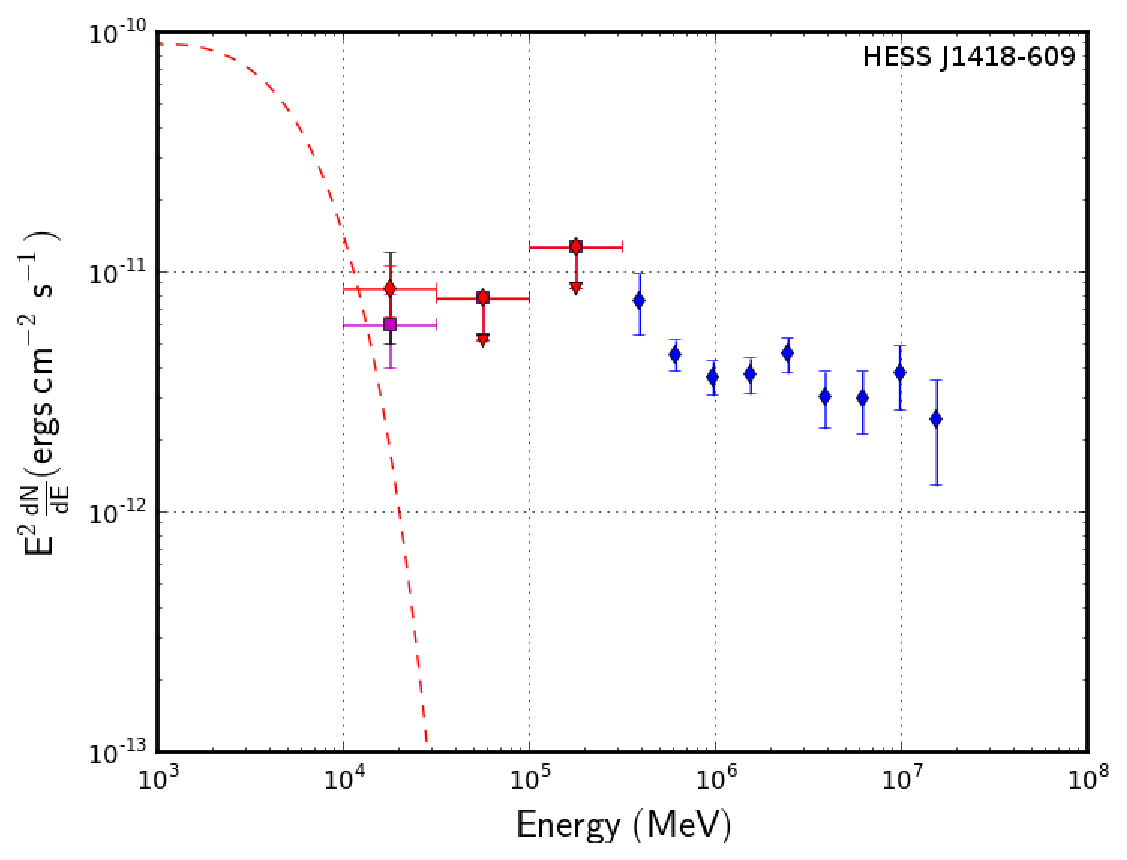
\includegraphics[width=0.45\textwidth]{figures/HESSJ1418.eps}
\label{fig:hessj1418}
}
\subfigure{
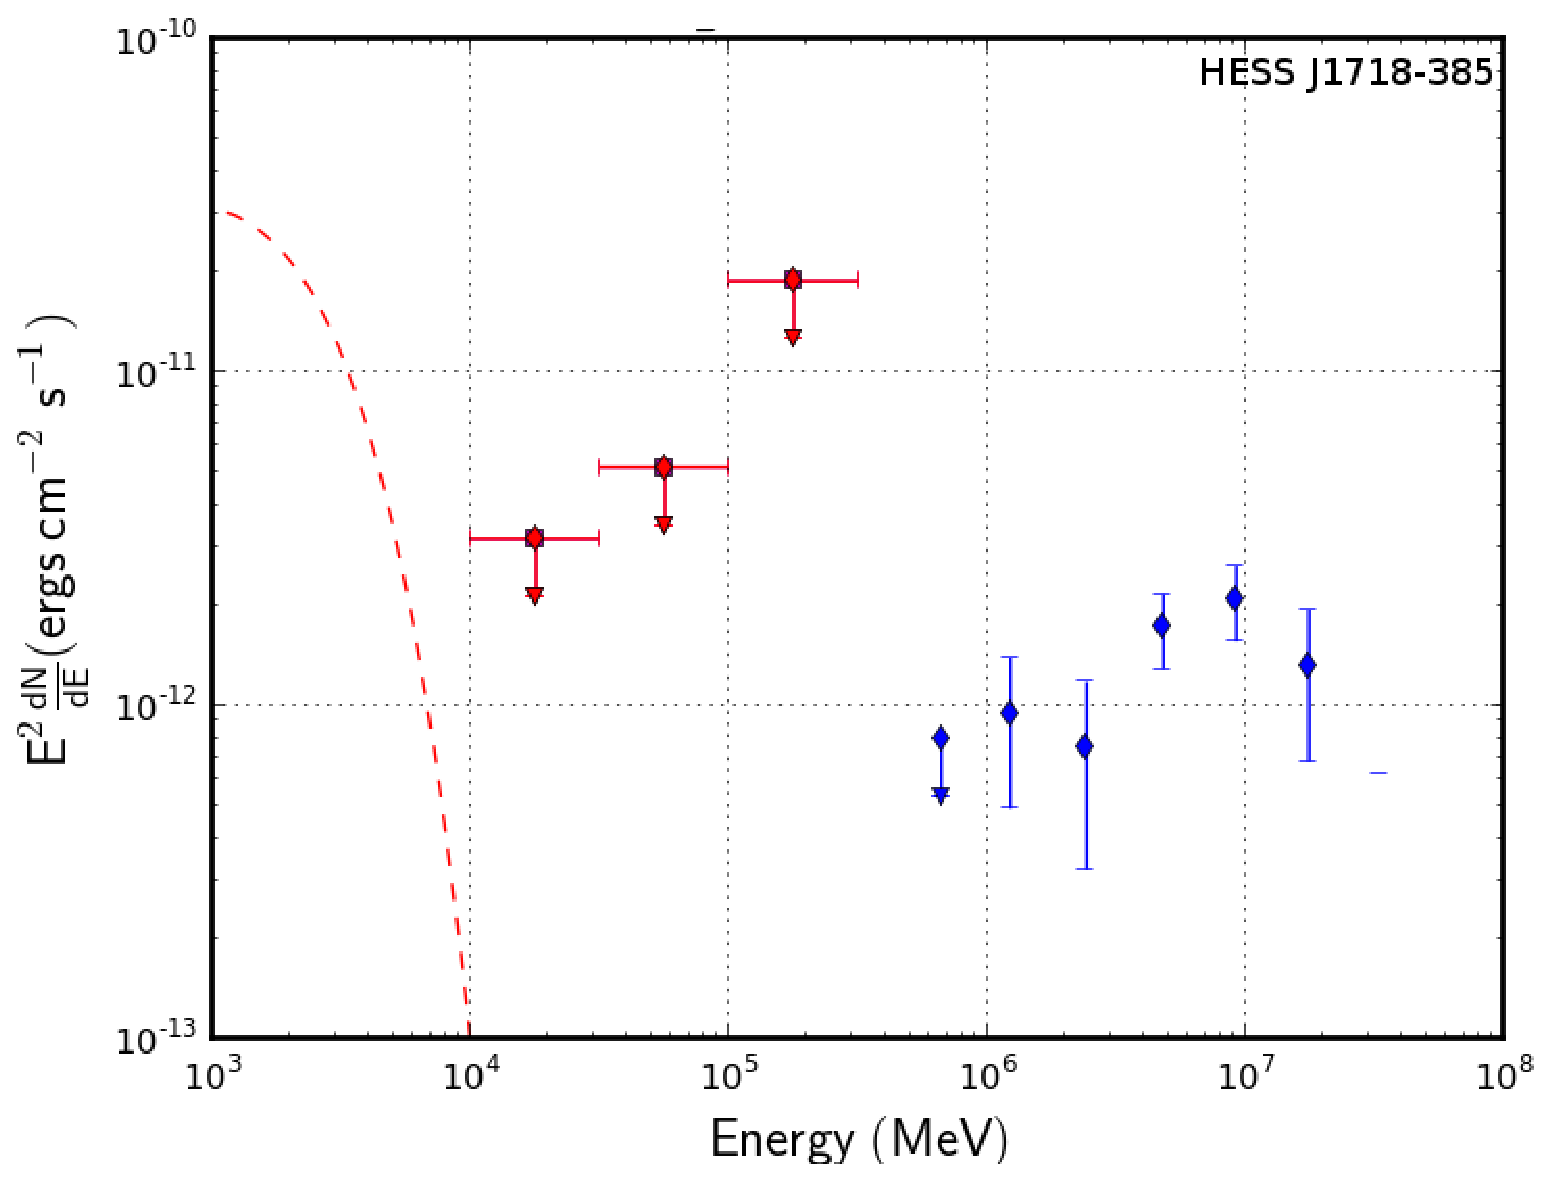
\includegraphics[width=0.45\textwidth]{figures/HESSJ1718.eps}
\label{fig:hessj1718}
}
\caption{\label{fig:sedsourcespuls2}SED of sources better described by the TeV shape and with a pulsar within 0.5$\degr$. The blue points show the TeV points taken from the associated paper in Table \ref{tab:TeV_sources}. The red circles and the magenta squares show respectively the SED without the pulsar included in the model and with the pulsar included in the model. The black error bars show the statistical and   systematic uncertainties added in quadrature. The dashed line corresponds to the model of the associated pulsars sumarized in Table \ref{tab:pulsarfit}.}
\end{figure}

\begin{figure}[h!]
\centering

\subfigure{
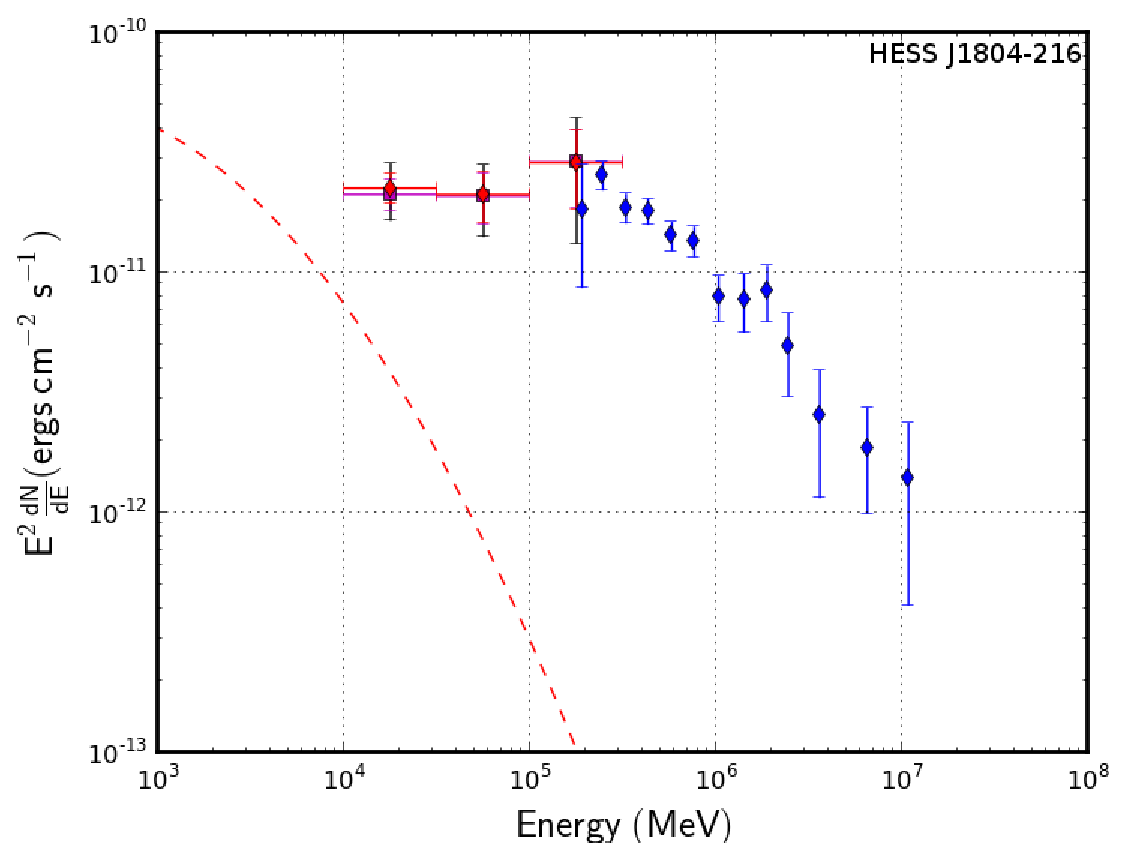
\includegraphics[width=0.45\textwidth]{figures/HESSJ1804.eps}
\label{fig:hessj1804}
}
\subfigure{
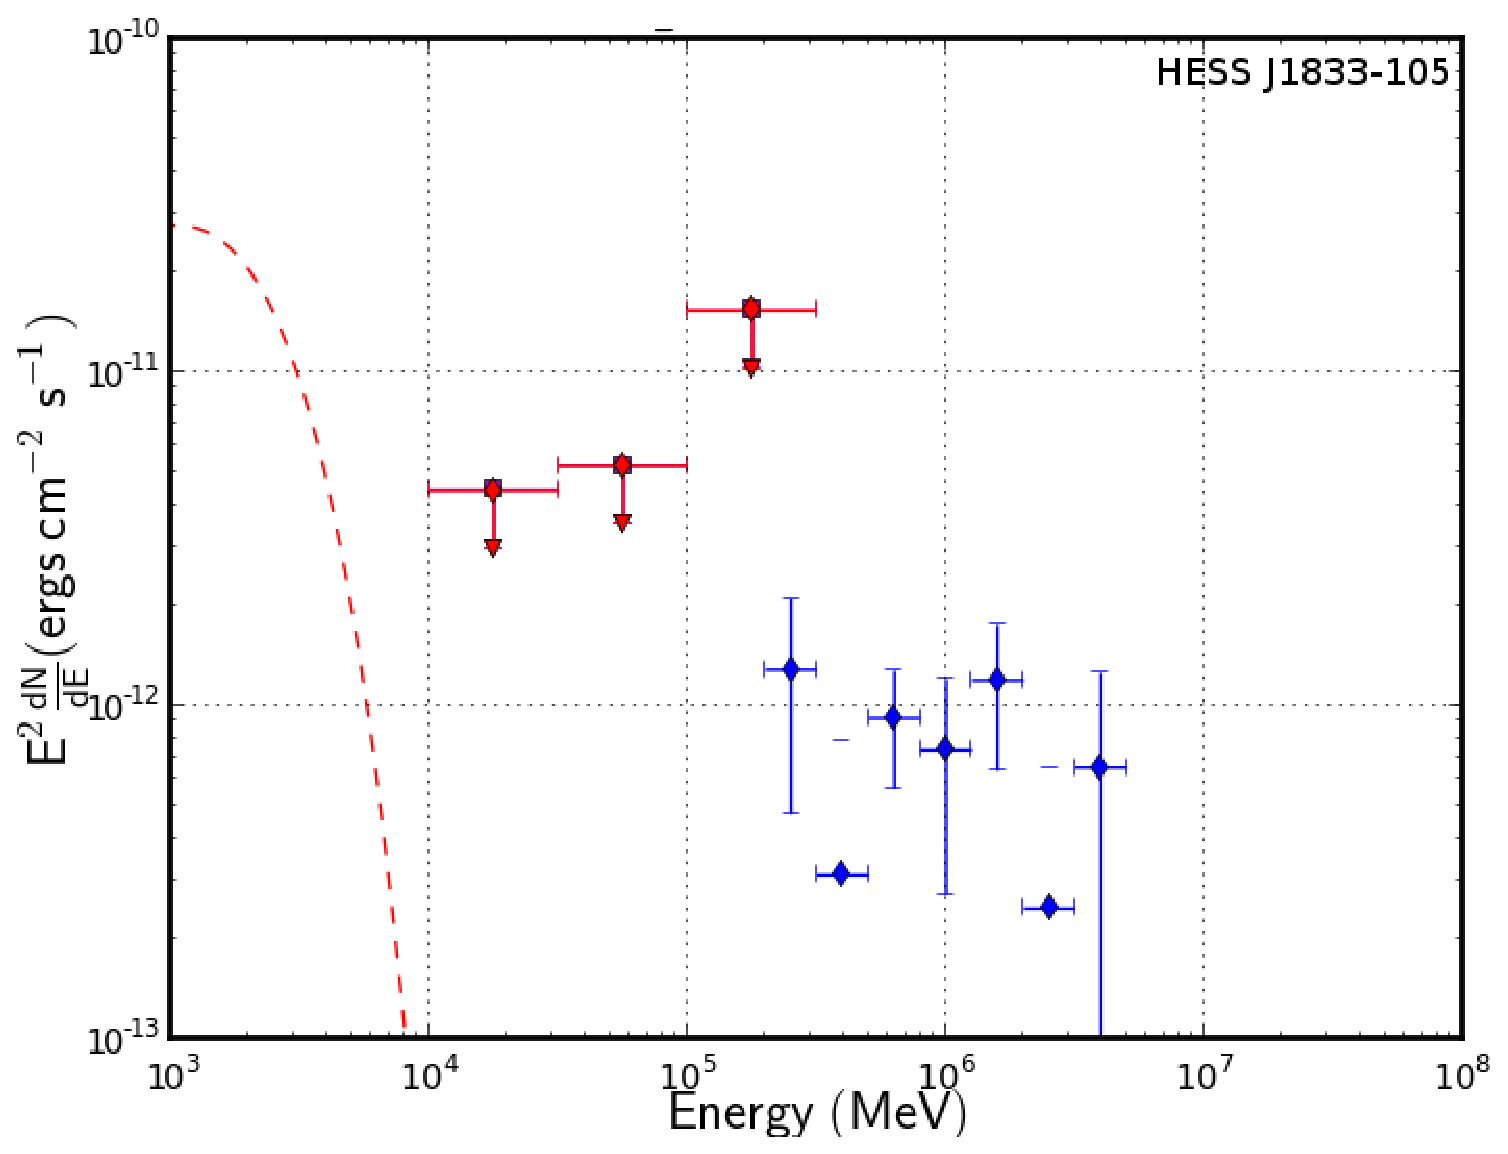
\includegraphics[width=0.45\textwidth]{figures/HESSJ1833.eps}
\label{fig:hess1833}
}
\subfigure{
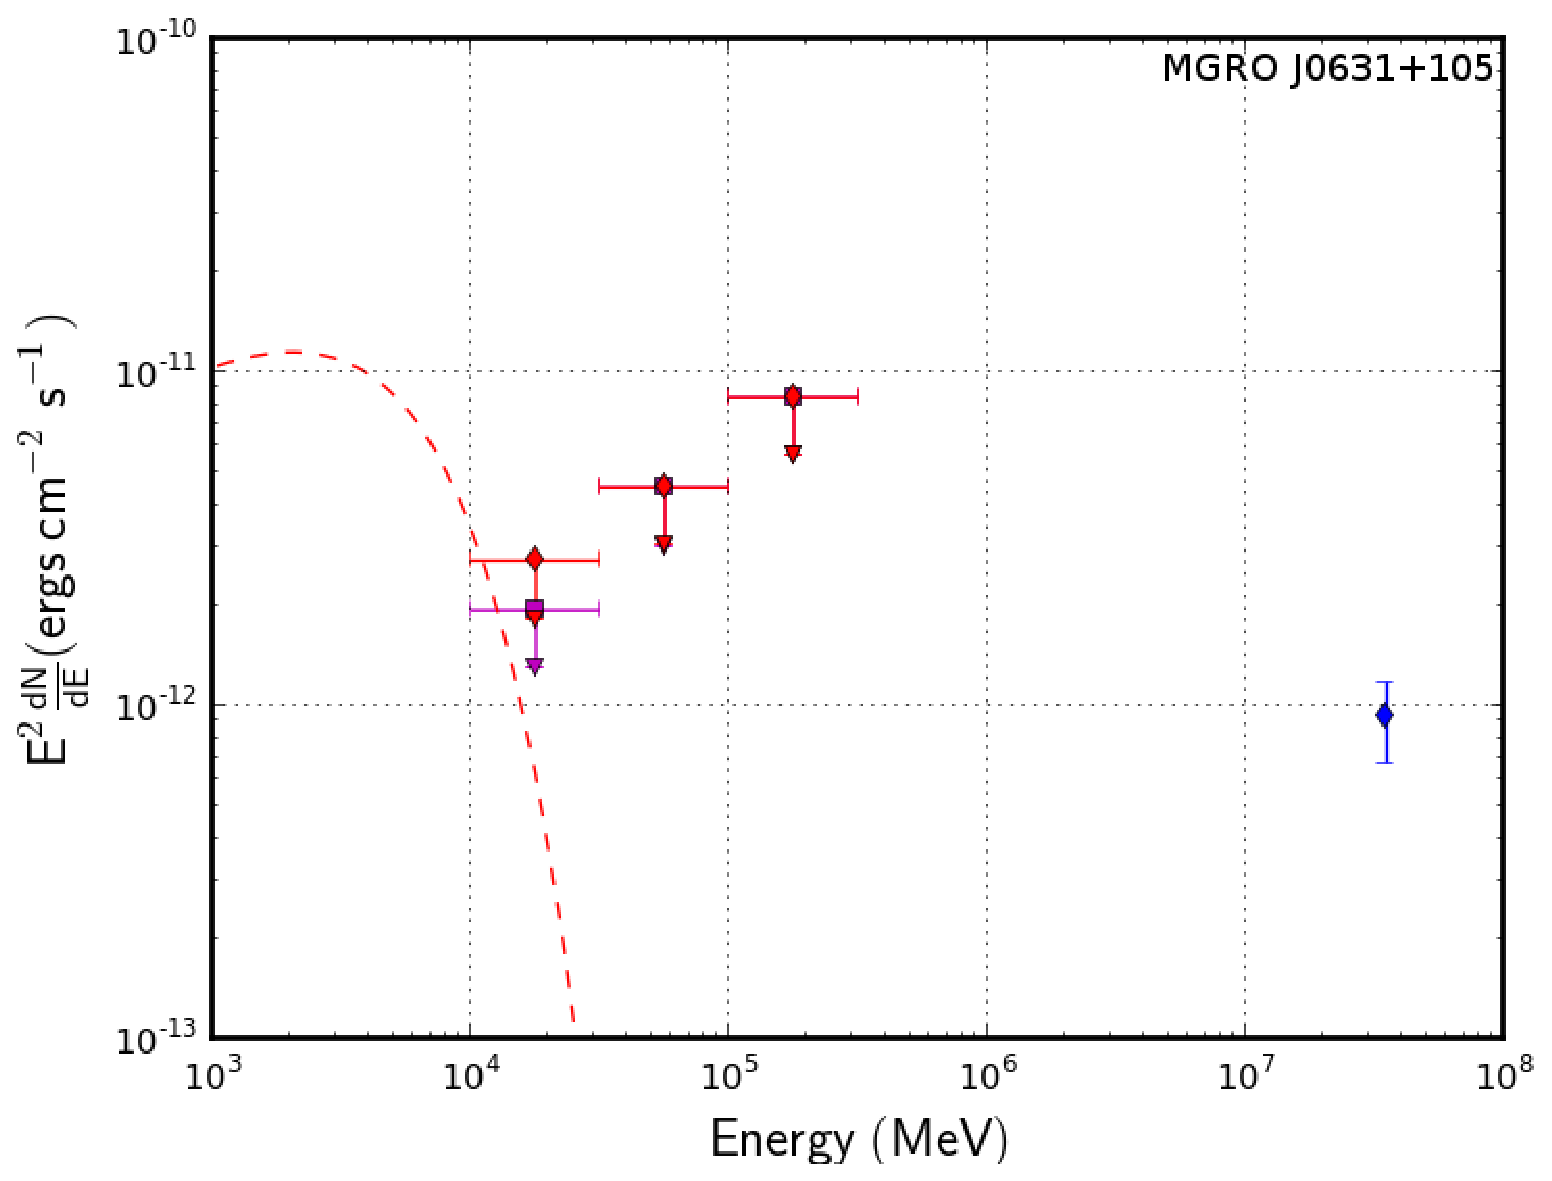
\includegraphics[width=0.45\textwidth]{figures/MGROJ0631.eps}
\label{fig:mgroj0631}
}
\subfigure{
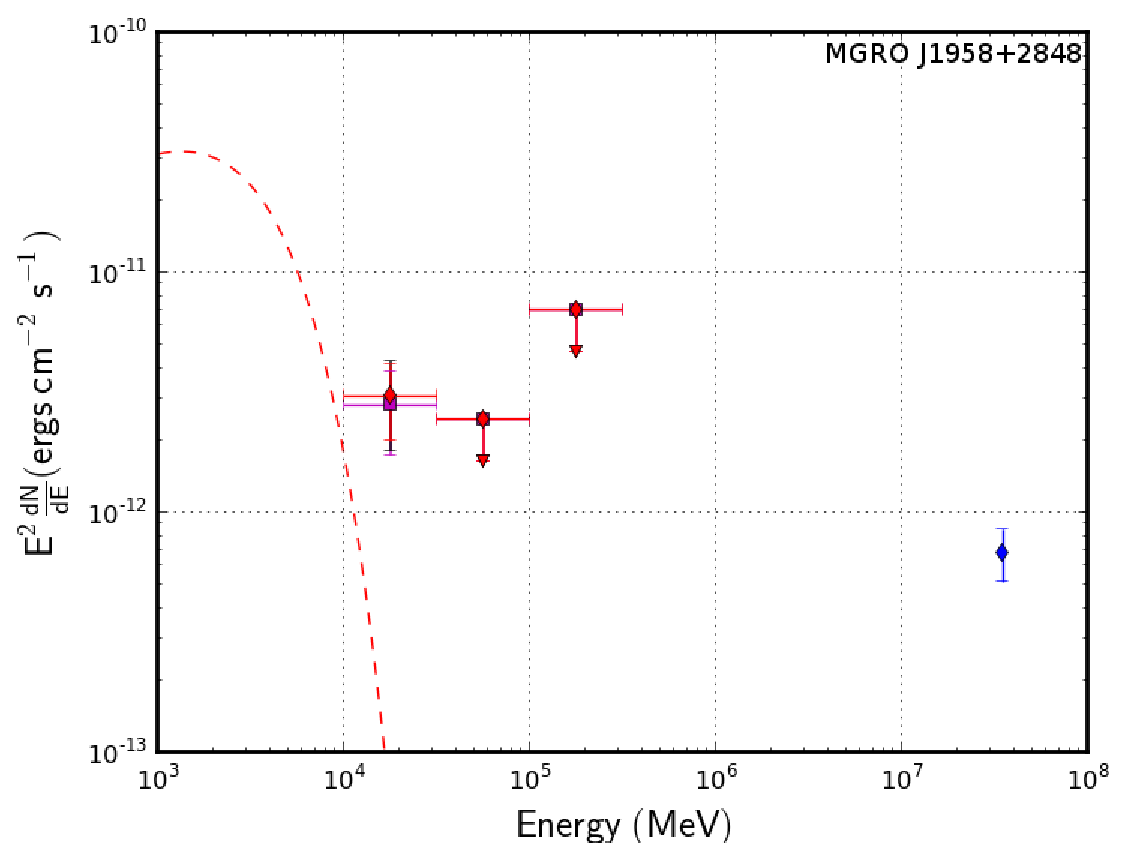
\includegraphics[width=0.45\textwidth]{figures/MGROJ1958.eps}
\label{fig:mgroj1958}
}

\caption{\label{fig:sedsourcespuls3}SED of sources better described by the TeV shape and with a pulsar within 0.5$\degr$. The blue points show the TeV points taken from the associated paper in Table \ref{tab:TeV_sources}. The red circles and the magenta squares show respectively the SED without the pulsar included in the model and with the pulsar included in the model. The black error bars show the statistical and   systematic uncertainties added in quadrature. The dashed line corresponds to the model of the associated pulsars summarized in Table. \ref{tab:pulsarfit}.}
\end{figure}

\clearpage

\begin{figure}[h!]
\centering
\subfigure{
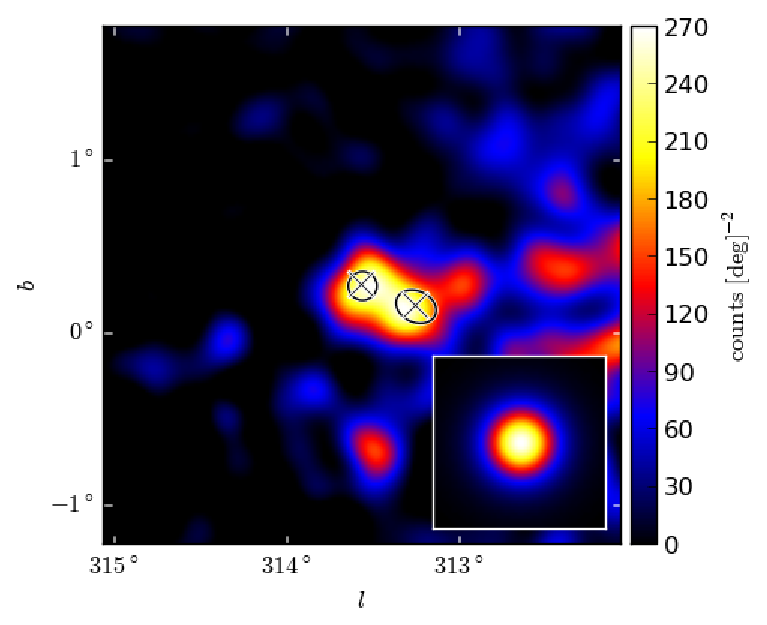
\includegraphics[width=0.60\textwidth]{figures/K310GeV.eps}}
\subfigure{
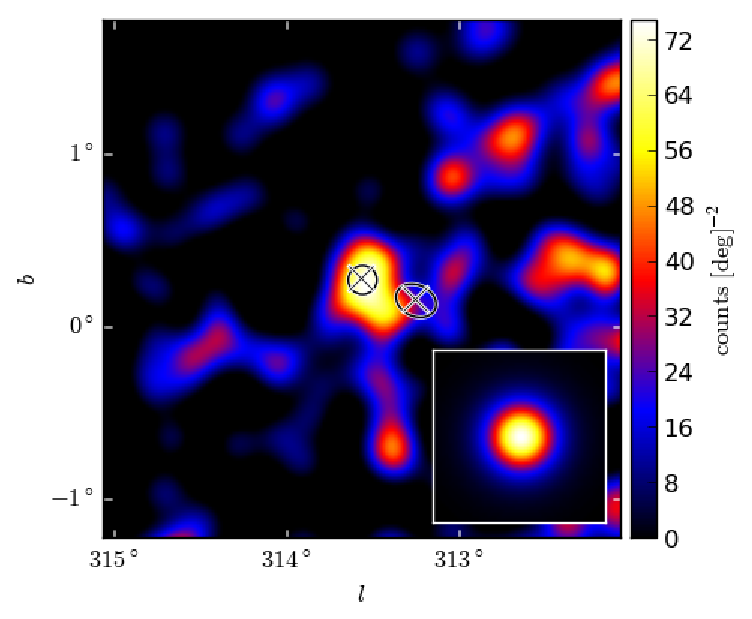
\includegraphics[width=0.60\textwidth]{figures/K330GeV.eps}}
\caption{Smoothed counts map of the region of the Kookaburra complex observed by Fermi above 10 GeV (Top) and
30 GeV (Bottom). The Galactic diffuse emission is subtracted. The circle and right ellipse show the best fit obtained in TeV respectively for the K3 nebula and the Rabbit nebula.
\label{fig:K3countsmap}}
\end{figure}

\clearpage

\begin{figure}[h!]
\centering
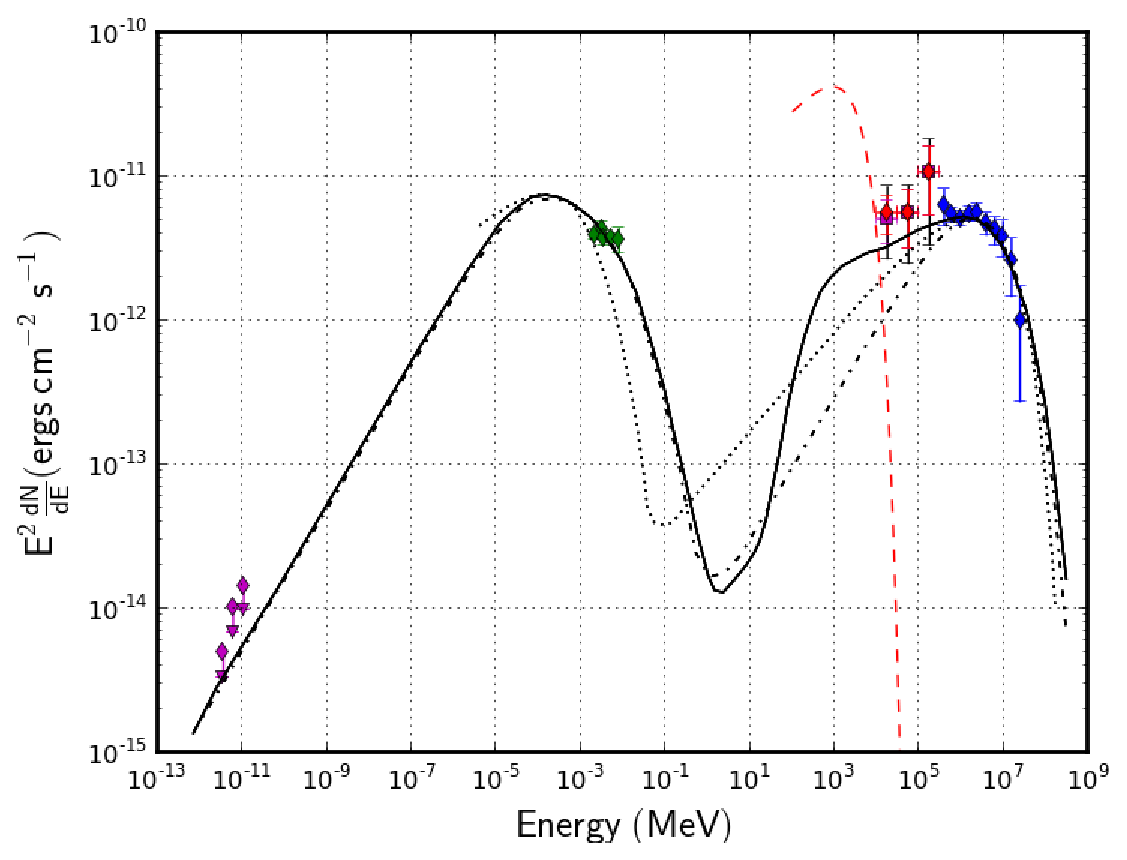
\includegraphics[width=0.60\textwidth]{figures/HESSJ1420.eps}
\caption{SED of HESS J1420-607. The blue, green and magenta points respectively show the spectral points obtained by HESS \citep{2006AA...456..245A}, by Suzaku \citep{2010ApJ...711.1168V} and the upper limits derived in radio. The red points and the magenta squares show the spectral points obtained in this work without and with the pulsar included in the model. In the LAT energy range the black error bars show the statistical and systematic uncertainties added in quadrature. The red dashed line corresponds to the 2FGL spectrum of the PSR J1420-607. The three black lines show the results of SED modeling for the broad extended nebula emission presented in previous works. The solid and dot dashed lines respectively shows to the hadronic plus leptonic and leptonic models proposed by \cite{2010ApJ...711.1168V}. The dotted line corresponds to the leptonic model proposed by \cite{2012ApJ...750..162K} assuming an ambient magnetic field of 3$\mu$G.
\label{fig:hessj1420}}
\end{figure}

\begin{figure}[h!]
\centering
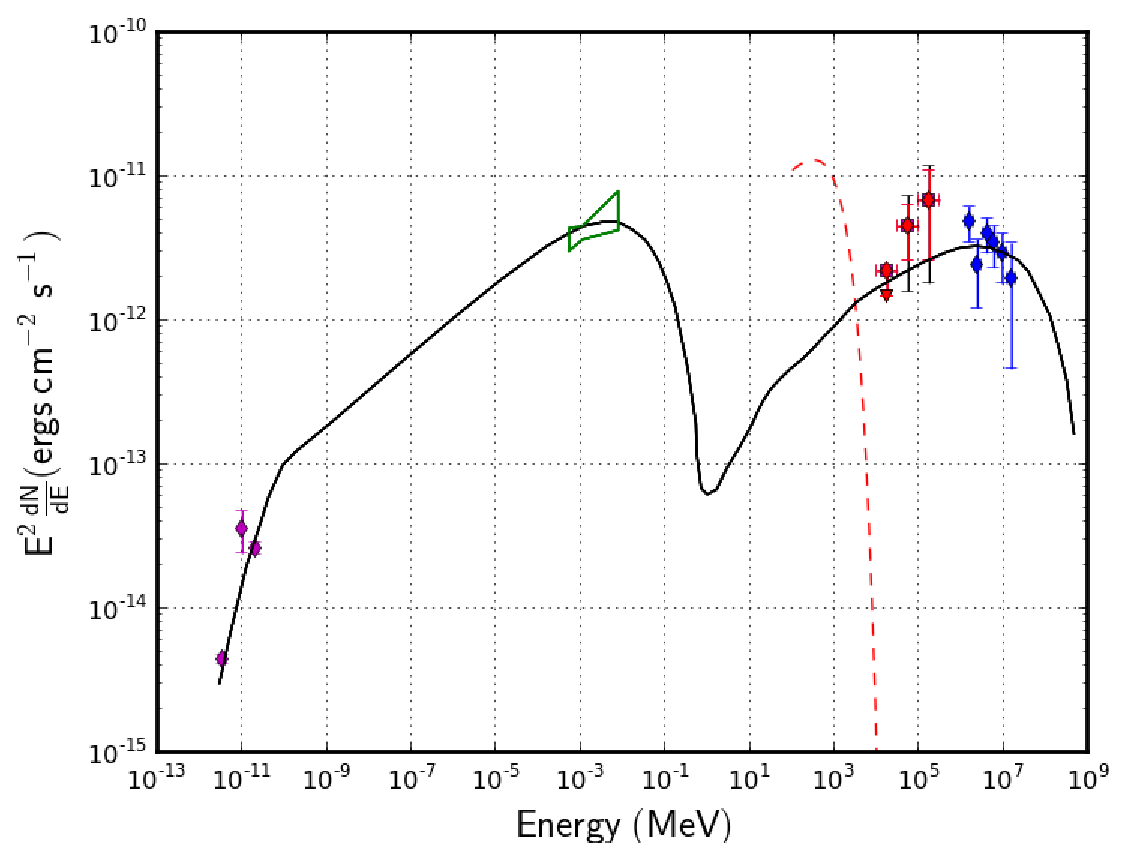
\includegraphics[width=0.60\textwidth]{figures/HESSJ1356.eps}
\caption{SED of HESS J1356-645. The blue, green and magenta points represents the results obtained by HESS \citep{2011AA...533A.103H}, the X-ray data \citep{2011AA...533A.102L} and the radio data \citep{2007MNRAS.382..382M, 1995MNRAS.277...36D, 1993AJ....105.1666G}. The red and magenta points between 10 and 316 GeV show the points obtained in this work without and with PSR J1357-6429 included in the model. In the LAT energy range the red and black error bars respectively show the statistical and systematic uncertainties added in quadrature. The solid line presents the one-zone leptonic model proposed by \cite{2011AA...533A.103H}.
\label{fig:hess1356}}
\end{figure}

\begin{figure}[h!]
\centering
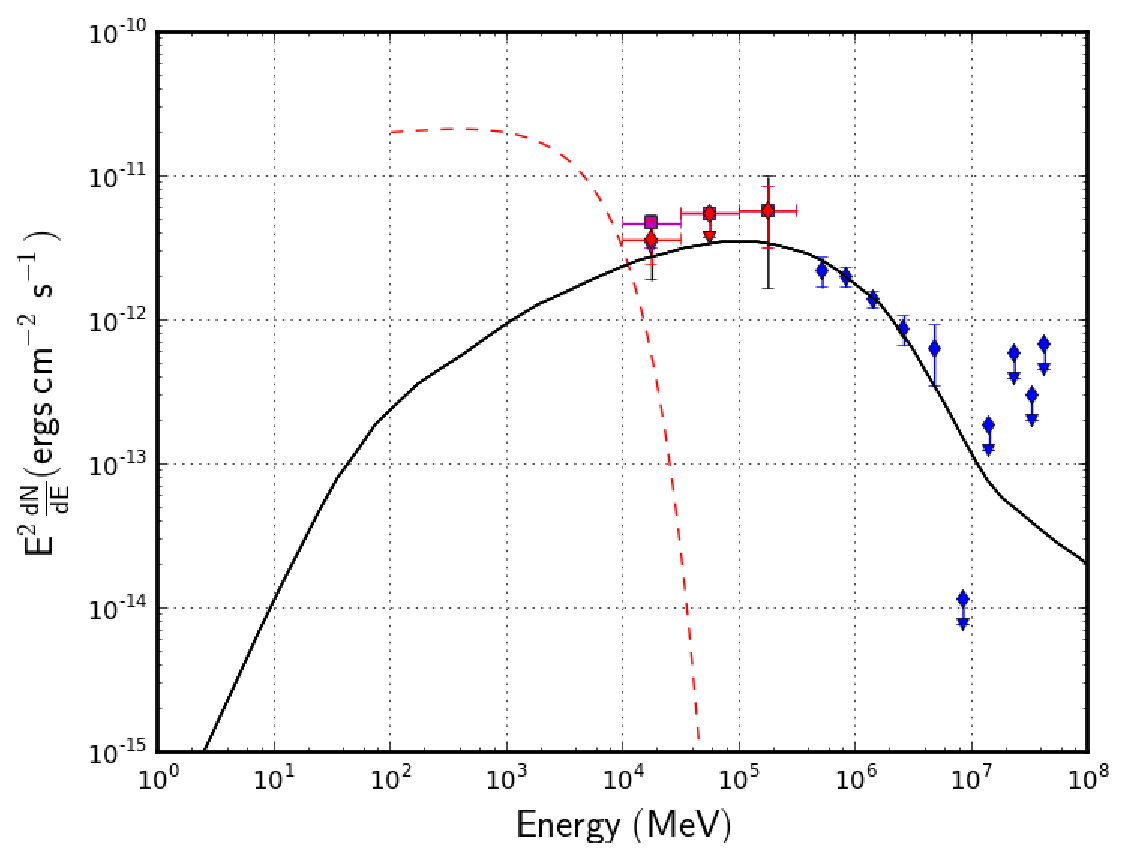
\includegraphics[width=0.60\textwidth]{figures/HESSJ1119.eps}
\caption{SED of HESS J1119$-$614. The blue points represent the HESS data \citep{Mayerdiploma}. The red and magenta points between 10 and 316 GeV show the points obtained in this work without and with PSR J1119$-$6127 included in the model. In the LAT energy range the red and black error bars respectively show the statistical and systematic uncertainties added in quadrature. The solid line shows the model proposed by \cite{Mayerdiploma}. The red dashed line corresponds to the model of PSR~J1119$-$6127 \citep{2012ApJS..199...31N}.
\label{fig:hessj1119}}
\end{figure}



\begin{figure}[h!]
\centering
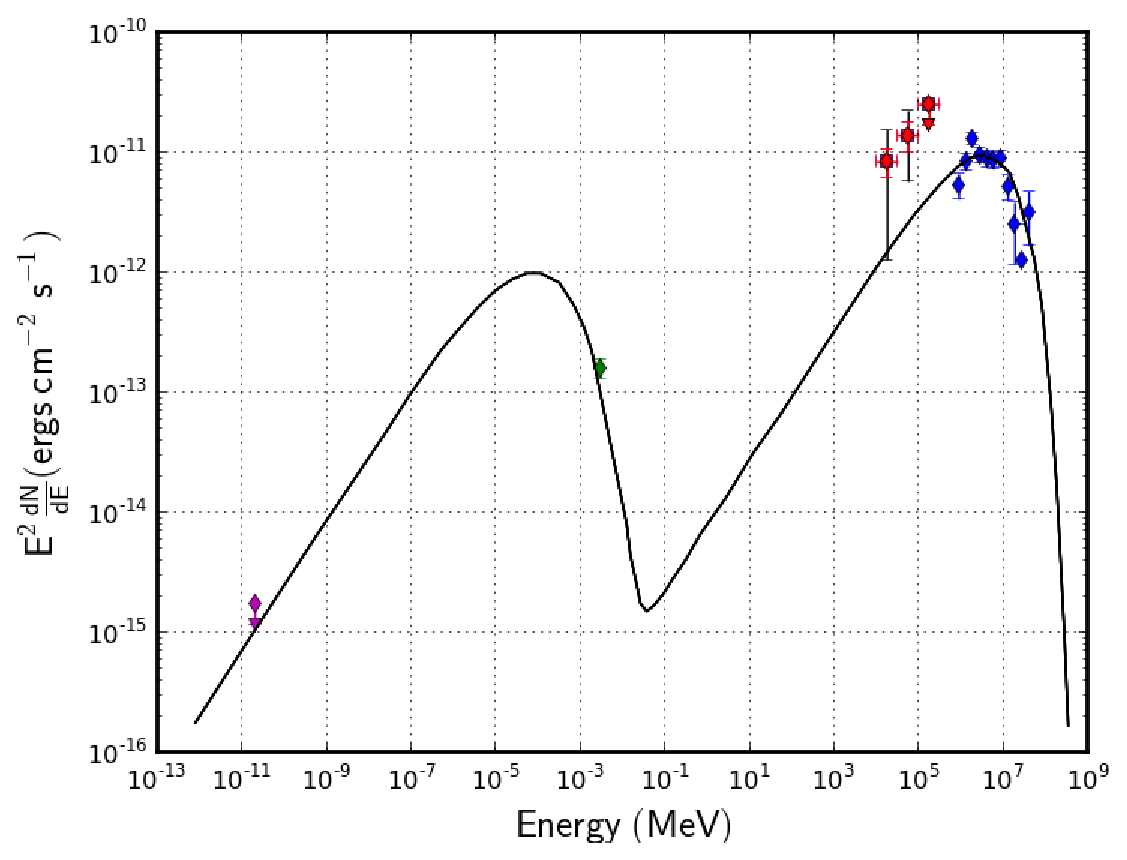
\includegraphics[width=0.60\textwidth]{figures/HESSJ1303631.eps}
\caption{SED of HESS J1303-631. The blue, green and magenta points represents HESS results, the radio data and \emph{Chandra} results \citep{dalton1303}. In the LAT energy range the red and black error bars respectively show the statistical and systematic uncertainties added in quadrature. The solid line shows the leptonic model proposed by \cite{dalton1303}.
\label{fig:hessj1303}}
\end{figure}


\begin{figure}[h!]
\centering
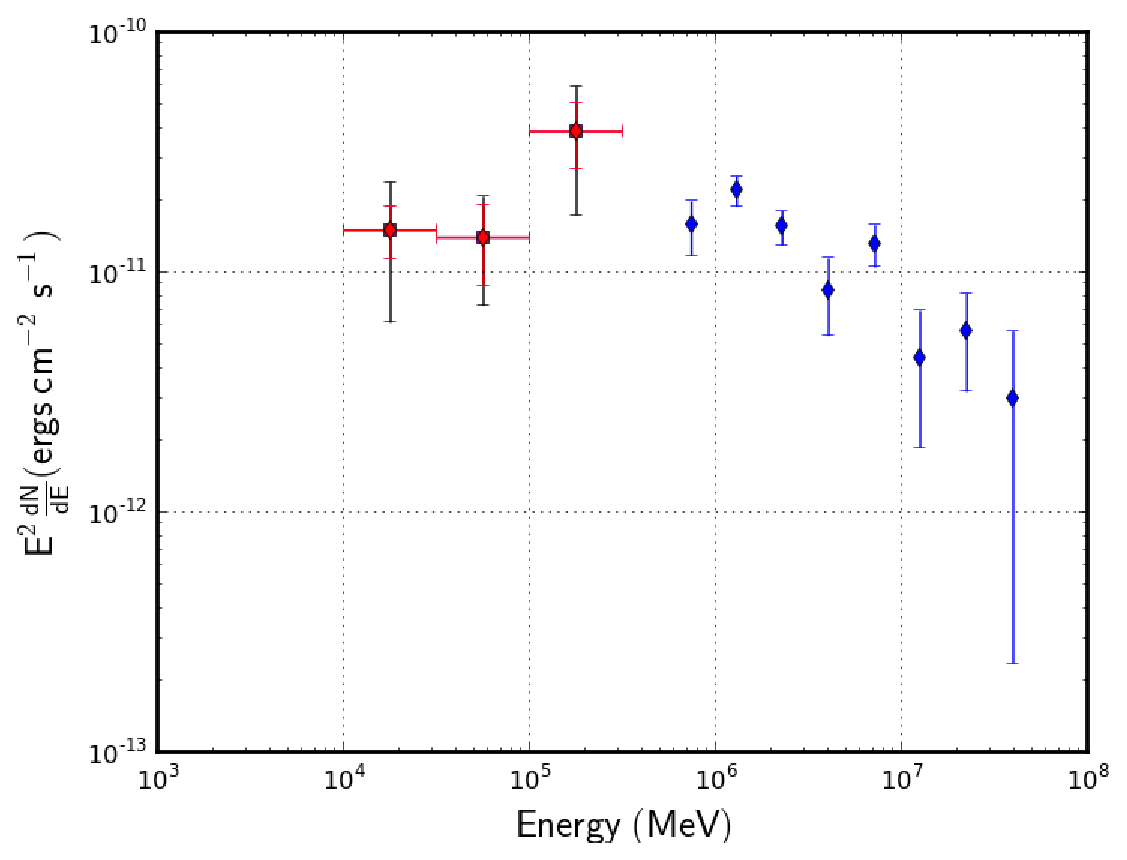
\includegraphics[width=0.60\textwidth]{figures/HESSJ1841055.eps}
\caption{SED of HESS~J1841$-$055. We reported the spectral points obtained using H.E.S.S. data in blues as well as the \emph{Fermi}-LAT spectral points in red. The red and black error bars respectively show the statistical and systematic uncertainties added in quadrature.
\label{fig:1841}}
\end{figure}

\begin{figure}[h!]
\centering
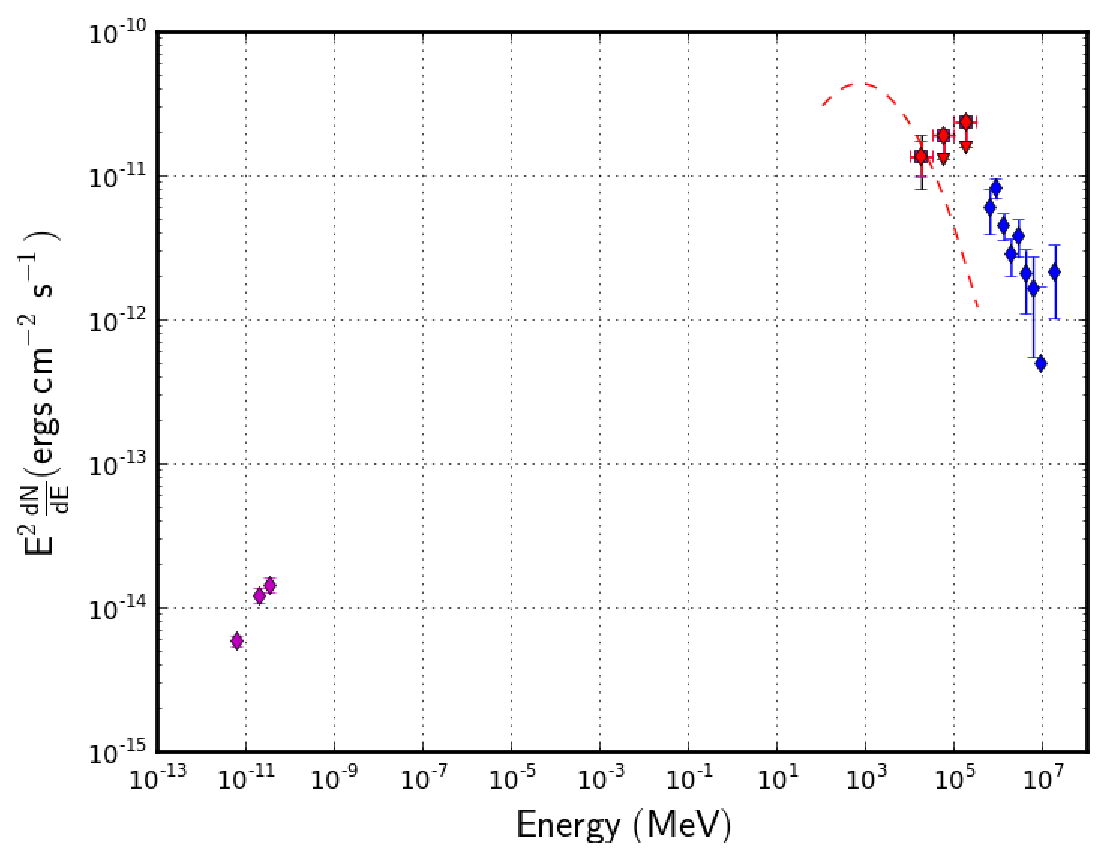
\includegraphics[width=0.60\textwidth]{figures/HESSJ1848018.eps}
\caption{SED of HESS~J1848$-$018. H.E.S.S. pectral points from \cite{chavesthesis} are presented in blue while the radio points corresponding to the W43 central cluster from \cite{2011AA...532A..92L} are indicated in magenta. Red points represent \emph{Fermi}-LAT data. The red and black error bars respectiveley show the statistical uncertainties and statistical plus systematic uncertainties added in quadrature. The red dashed line corresponds to the SED derived in \cite{2011MmSAI..82..739L} using \emph{Fermi}-LAT data and assuming a Gaussian shape of 0.3$\degr$.
\label{fig:1848}}
\end{figure}

\begin{figure}[h!]
\centering
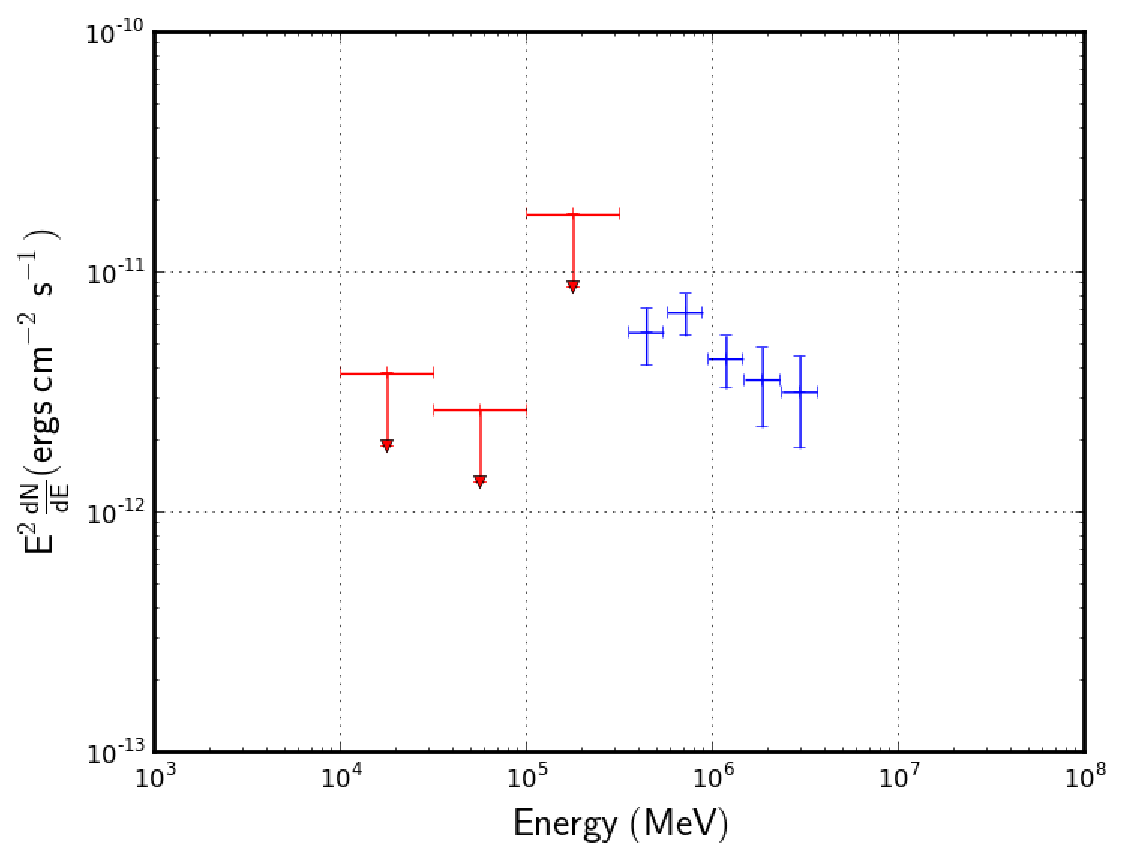
\includegraphics[width=0.60\textwidth]{figures/HESSJ1026.eps}
\caption{SED of HESS~J1026$-$582. H.E.S.S. spectral points are reported in blue while \emph{Fermi}-LAT upper limits are indicated in red. 
\label{fig:1026}}
\end{figure}

\begin{figure}[h!]
\centering
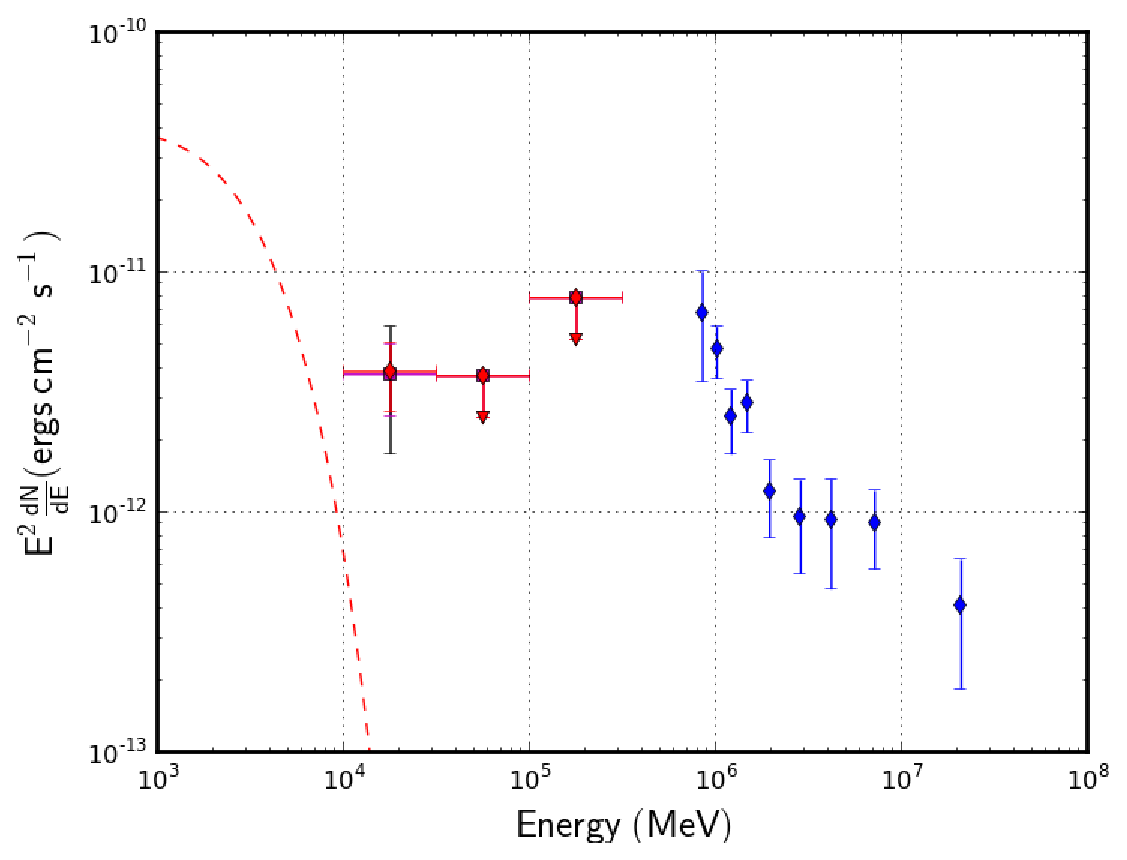
\includegraphics[width=0.60\textwidth]{figures/HESSJ1458.eps}
\caption{SED of HESS~J1458$-$608. H.E.S.S. spectral points are reported in blue while \emph{Fermi}-LAT spectral points are represented int red. The magenta points show the \emph{Fermi}-LAT points obtained once PSR~J1459$-$60 added to the model. The black error bars show the statistical and systematic uncertainties added in quadrature.
\label{fig:1458}}
\end{figure}

\begin{figure}[h!]
\centering
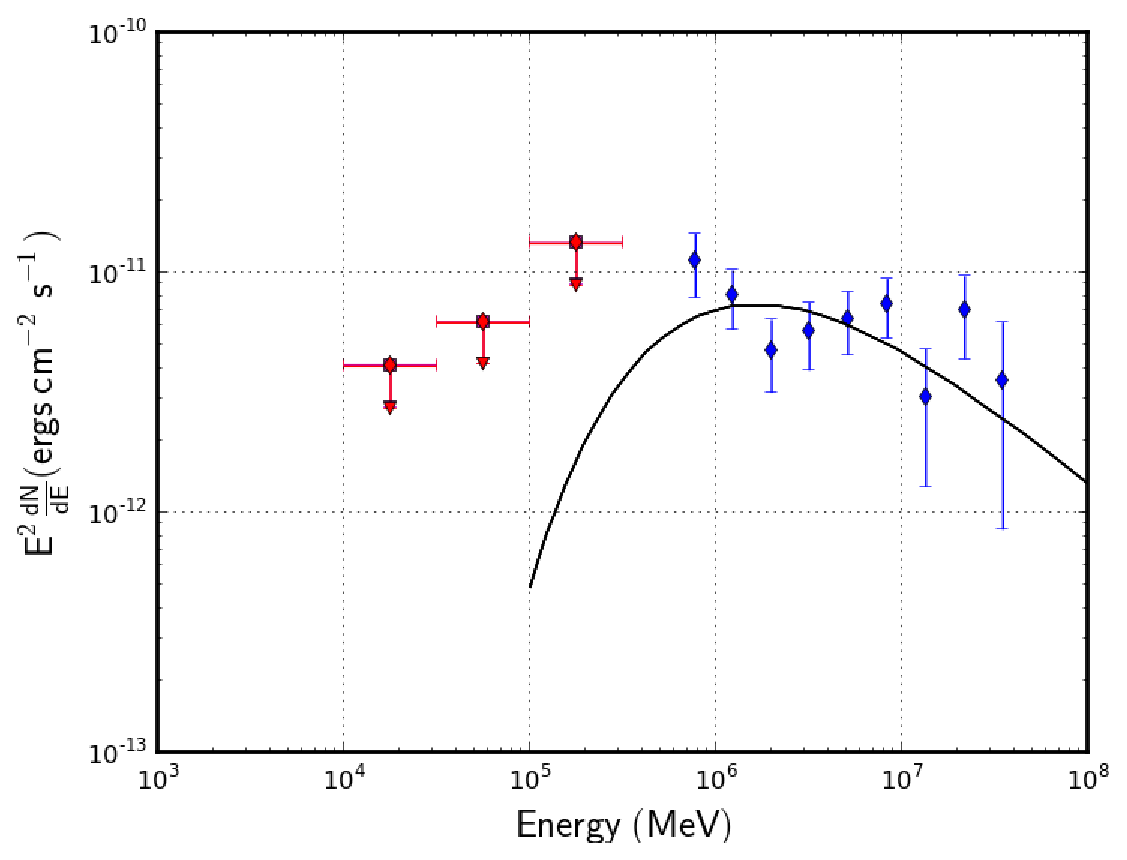
\includegraphics[width=0.60\textwidth]{figures/HESSJ1626.eps}
\caption{SED of HESS~J1626$-$490. H.E.S.S. spectral points are reported in blue while \emph{Fermi}-LAT upper-limits are indicated in red.
\label{fig:1626}}
\end{figure}

\begin{figure}[h!]
\centering
\subfigure{
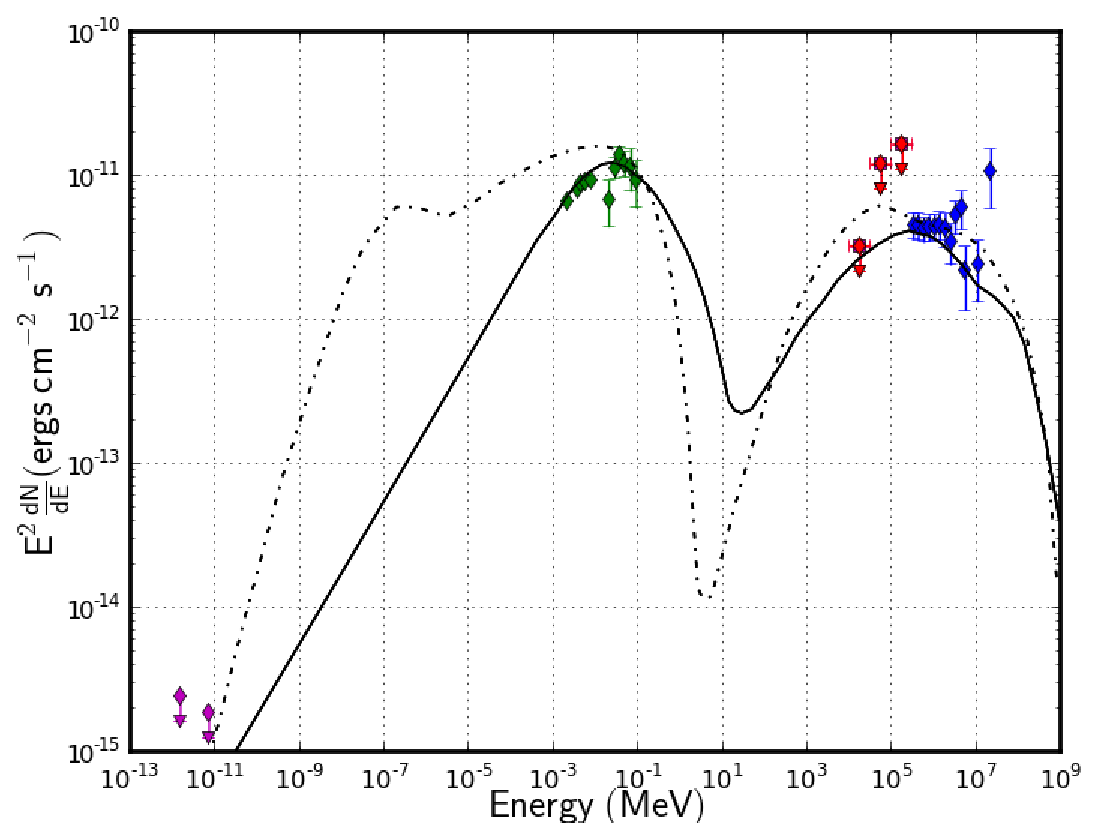
\includegraphics[width=0.60\textwidth]{figures/HESSJ1813178PWN.eps}}
\subfigure{
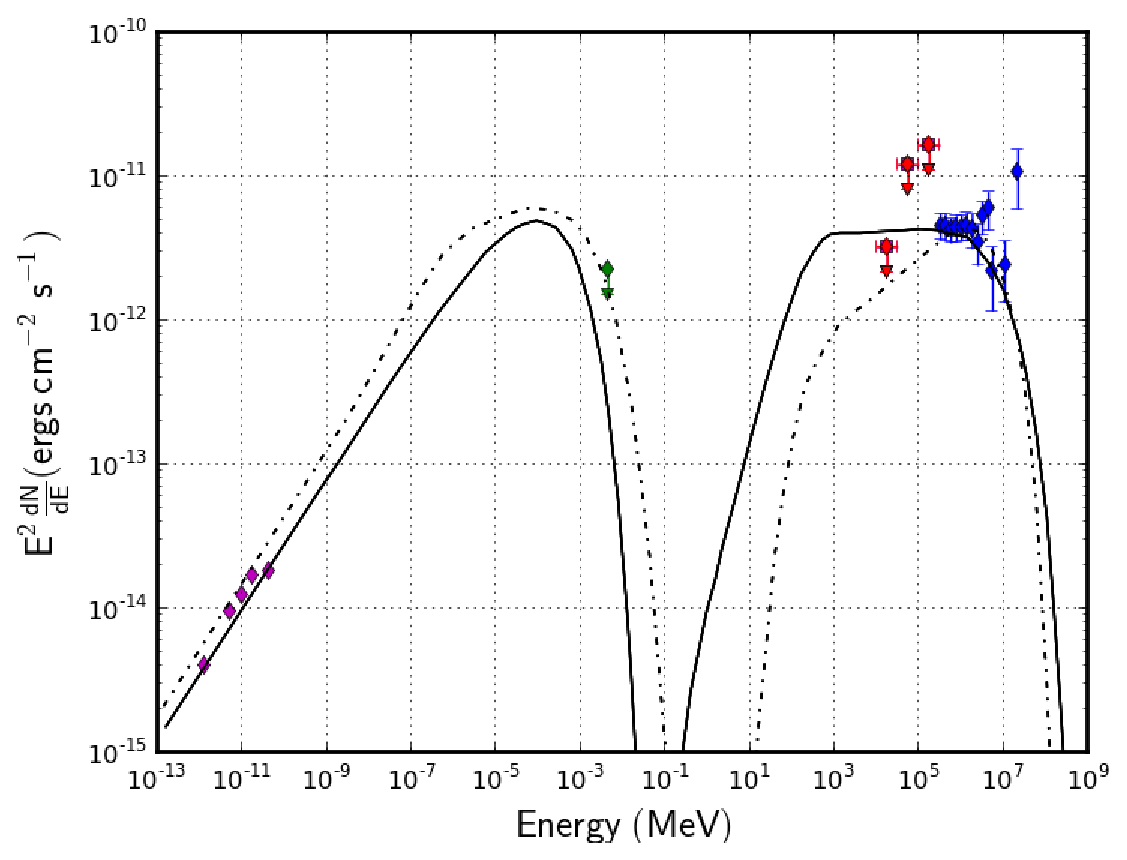
\includegraphics[width=0.60\textwidth]{figures/HESSJ1813178SNR.eps}}
\caption{SED of HESS J1813$-$178. The blue and red points show the H.E.S.S. \citep{2006ApJ...636..777A} and \emph{Fermi}-LAT spectral results. The radio data (magenta) are from VLA, Bonn, Parkes, and Nobeyama observatories \citep{2005ApJ...629L.105B}. The X-ray data are from XMM-Newton \citep{2007AA...470..249F}
and INTEGRAL \citep{2005ApJ...629L.109U}. These points were derived either for the shell of the SNR and for the core (PWN). The solid and dot dashed lines respectively correspond to the models proposed by \cite{2007AA...470..249F} and by \cite{2010ApJ...718..467F}. Top : Leptonic scenario in which the radiation is created by a PWN.  Bottom : Hadronic scenario in which the radiation is created by the SNR. 
\label{fig:hessj1813}}
\end{figure}




\clearpage

\begin{figure}[h!]
\centering
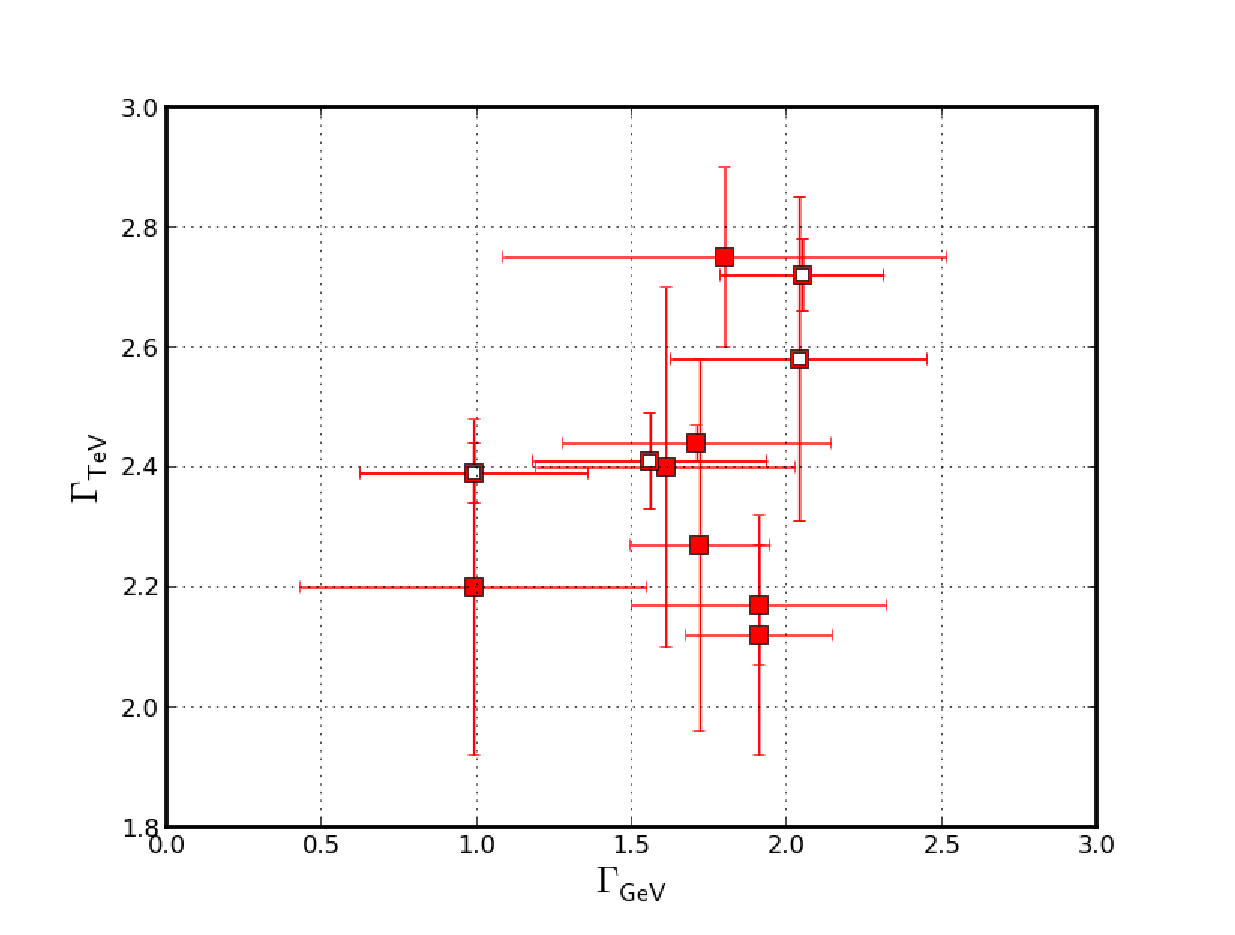
\includegraphics[width=0.5\textwidth]{figures/Gamma_GeV_Gamma_TeV.eps}
\caption{TeV spectral index as a function of the GeV spectral index for sources detected in our analysis for which the informations on the pulsar are available. These sources are summarized in Table \ref{tab:table_luminosity}. Full markers represent sources with a clear PWN association at TeV energies while hollow markers correspond to sources for which the association between TeV emission and a PWN is less clear. The dashed line corresponds to the symmetry compared to an index of 2. Pulsars summarized in Table \ref{tab:pulsarfit} are included in the model.
\label{fig:gammagamma}}
\end{figure}

\begin{figure}[h!]
\centering
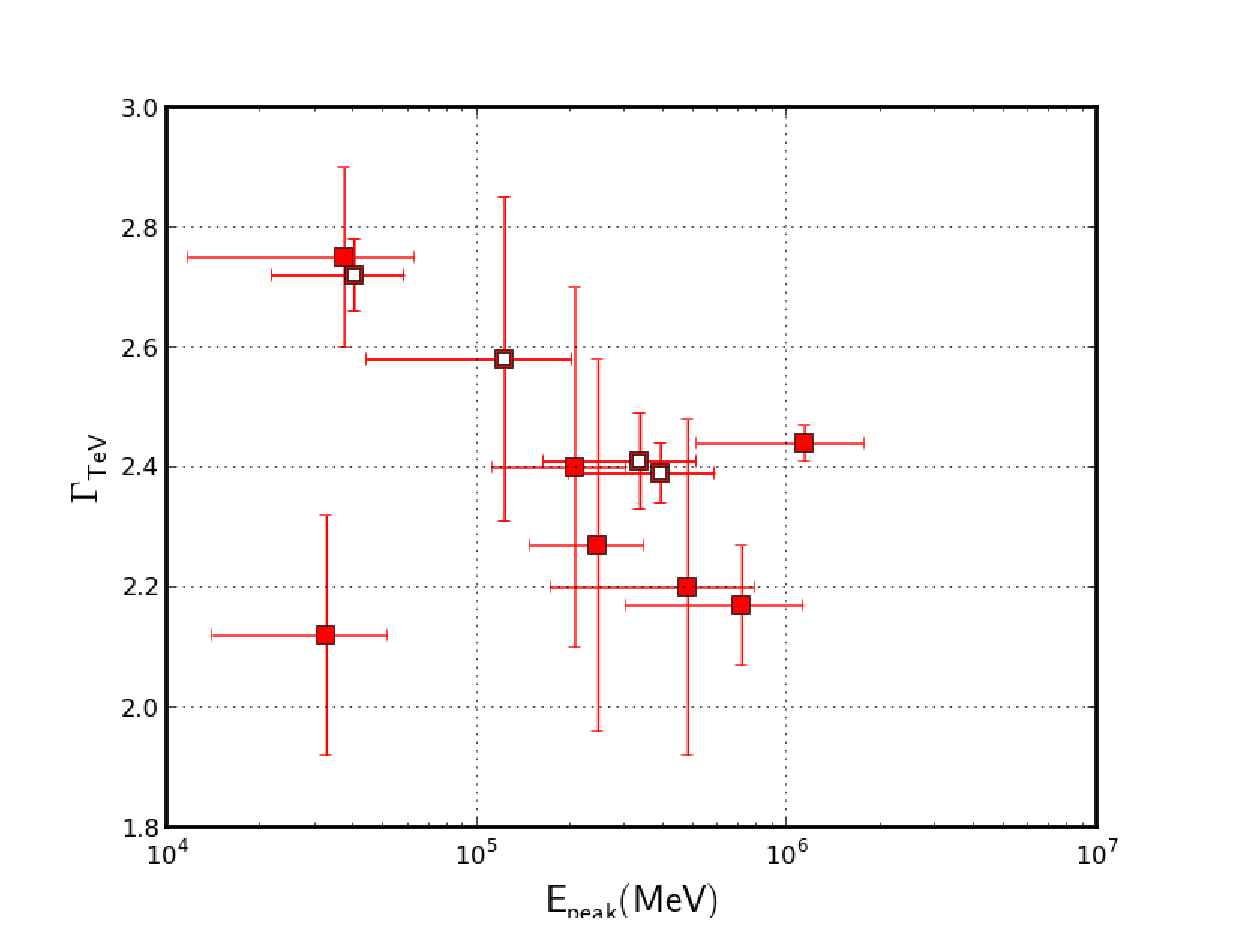
\includegraphics[width=0.5\textwidth]{figures/E_cut_vs_TeV.eps}
\caption{TeV spectral index as a function of the energy of the maximum of the IC peak for sources detected in our analysis for which the informations on the pulsar are available. These sources are summarized in Table \ref{tab:table_luminosity}. Full markers represent sources with a clear PWN association at TeV energies while hollow markers correspond to sources for which the association between TeV emission and a PWN is less clear. Pulsars summarized in Table \ref{tab:pulsarfit} are included in the model.
\label{fig:EpeakETeV}}
\end{figure}

\begin{figure}[h!]
\centering
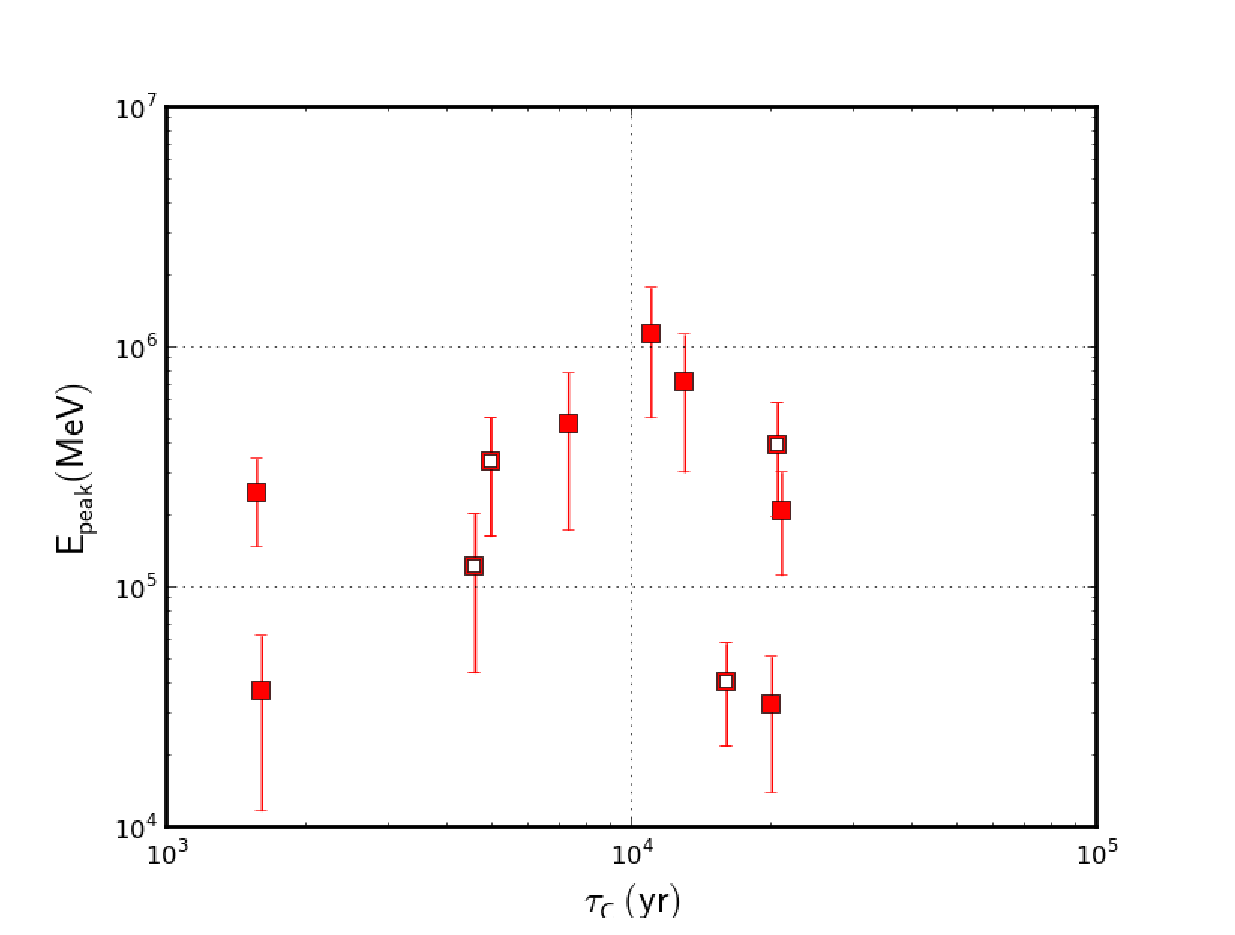
\includegraphics[width=0.5\textwidth]{figures/E_cut_vs_age.eps}
\caption{Energy of the maximum of IC peak as a function of the characteristic age of the pulsar for sources detected in our analysis for which the informations on the pulsar are available. These sources are summarized in Table \ref{tab:table_luminosity}. Full markers represent sources with a clear PWN association at TeV energies while hollow markers correspond to sources for which the association between TeV emission and a PWN is less clear. Pulsars summarized in Table \ref{tab:pulsarfit} are included in the model.
\label{fig:Epeakage}}
\end{figure}

\clearpage

\begin{figure}[h!]
\centering
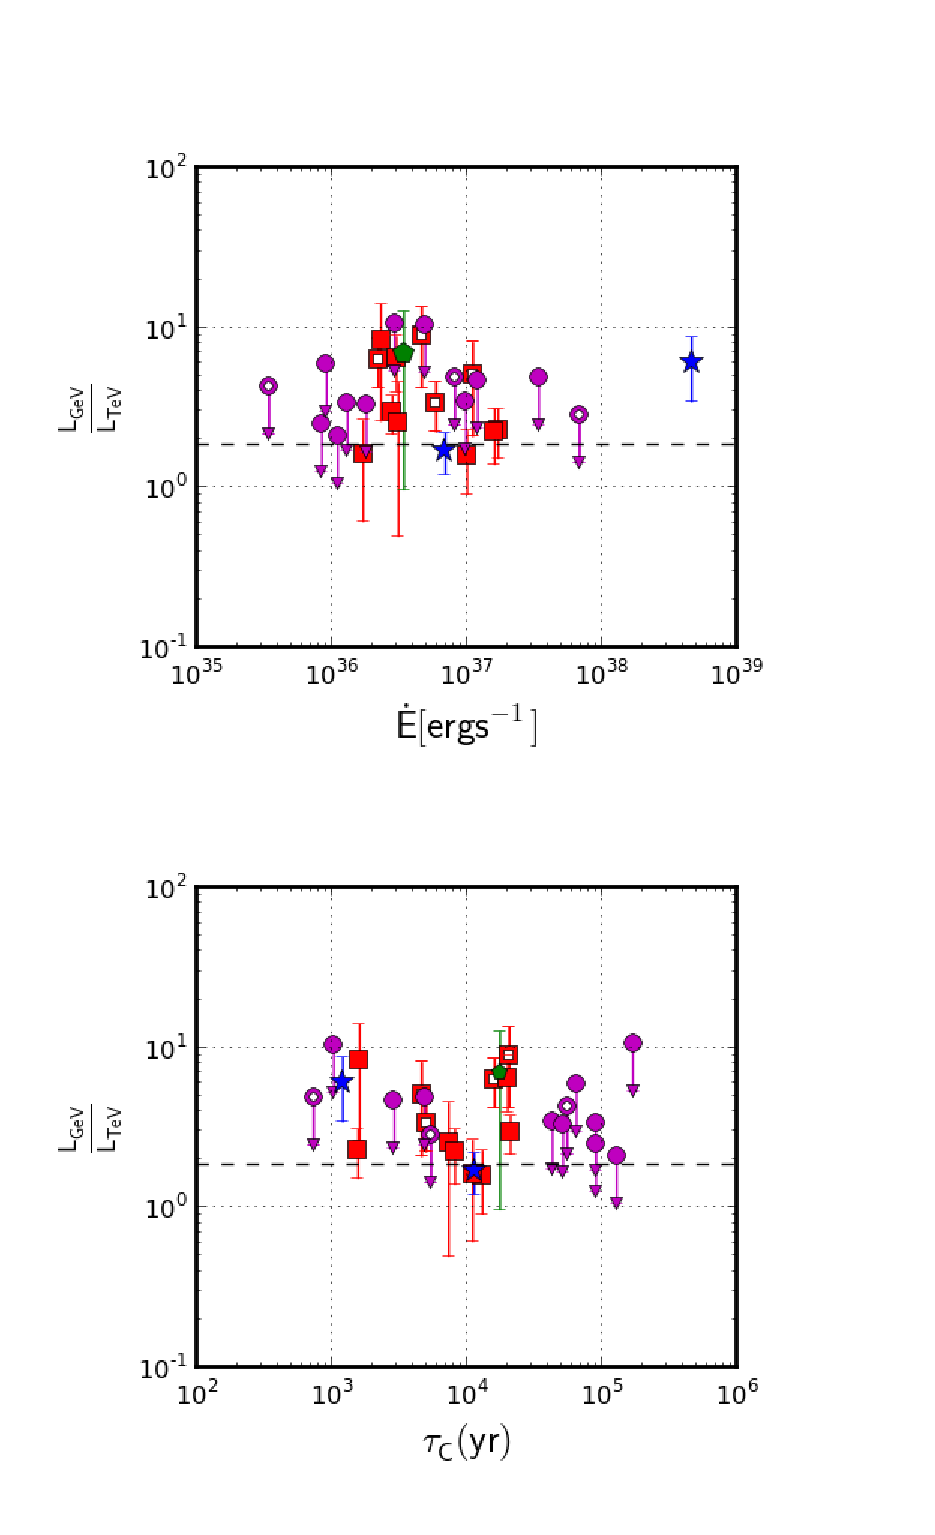
\includegraphics[width=0.5\textwidth]{figures/rapport_TeV.eps}
\caption{Ratio of luminosity of the PWN in GeV over the luminosity in TeV as a function of the pulsar spin-down power (top) and the pulsar characteristic age (bottom). Full markers correspond to sources with a clear PWN association at TeV energies while hollow markers correspond to sources for which the association between the TeV emission and a PWN is less clear. The red squares (\protect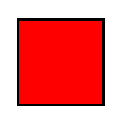
\includegraphics[scale=0.25]{figures/carrerouge.eps}) represent the sources detected at GeV energies, the magenta circles (\protect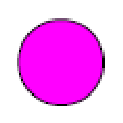
\includegraphics[scale=0.25]{figures/rondmagenta.eps}) show the upper limits, the green pentagon (\protect
\includegraphics[scale=0.25]{figures/pentagonevert.eps}) represent the sources showing a pulsar behaviour in the energy range and the blue stars (\protect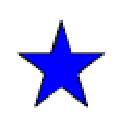
\includegraphics[scale=0.25]{figures/etoilebleue.eps}) represent the Crab nebula and Vela-X not studied in this work. Pulsars summarized in Table \ref{tab:pulsarfit} are included in the model. The dashed line represent the mean ratio found between the GeV and the TeV flux due to the spectral shape of the IC peak.
\label{fig:rapportTeV}}
\end{figure}

\clearpage

\begin{figure}[h!]
\centering
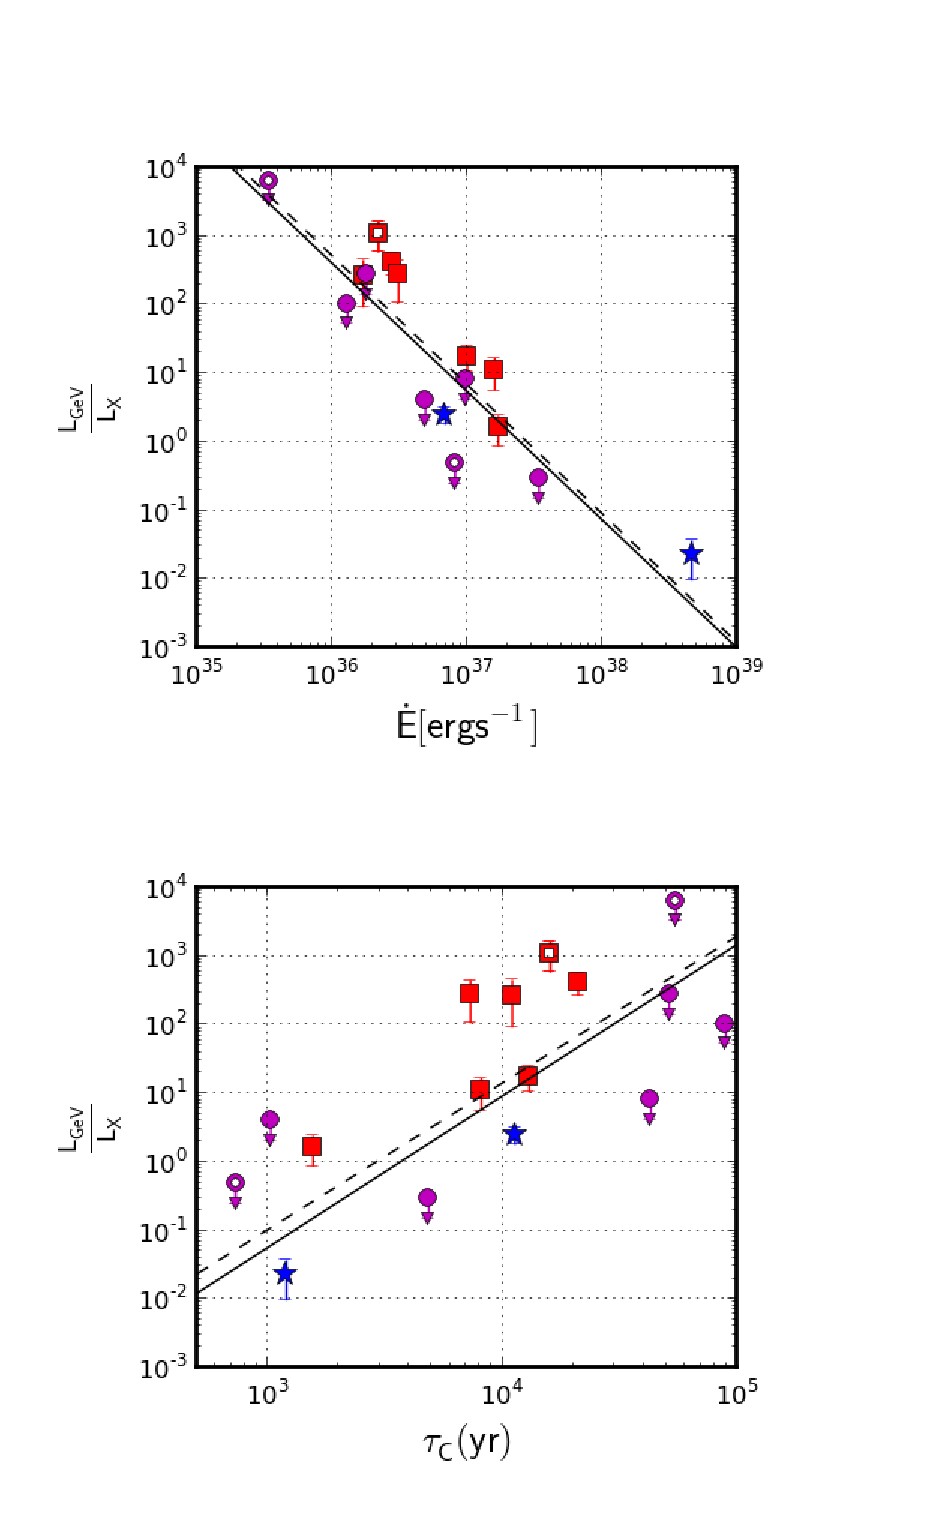
\includegraphics[width=0.5\textwidth]{figures/rapport_X.eps}
\caption{Ratio of luminosity of the PWN in GeV over the luminosity in X-rays as a function of the pulsar spin-down power (top) and the pulsar characteristic age (bottom). Full markers correspond to sources with a clear PWN association at TeV energies while hollow markers correspond to sources for which the association between the TeV emission and a PWN is less clear. The red squares (\protect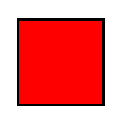
\includegraphics[scale=0.25]{figures/carrerouge.eps}) represent the sources detected at GeV energies, the magenta circles (\protect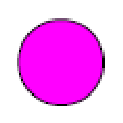
\includegraphics[scale=0.25]{figures/rondmagenta.eps}) show the upper limits, the green pentagon (\protect
\includegraphics[scale=0.25]{figures/pentagonevert.eps}) represent the sources showing a pulsar behaviour in the energy range and the blue stars (\protect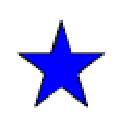
\includegraphics[scale=0.25]{figures/etoilebleue.eps}) represent the Crab nebula and Vela-X not studied in this work. Pulsars summarized in Table \ref{tab:pulsarfit} are included in the model. The dashed and solid lines represent respectively the relations derived in \cite{2009ApJ...694...12M} multiplied by $\bar{R}$ for the whole sample of sources and for the sources clearly identify to PWNe.
\label{fig:rapportX}}
\end{figure}

\clearpage

\begin{figure}[h!]
\centering
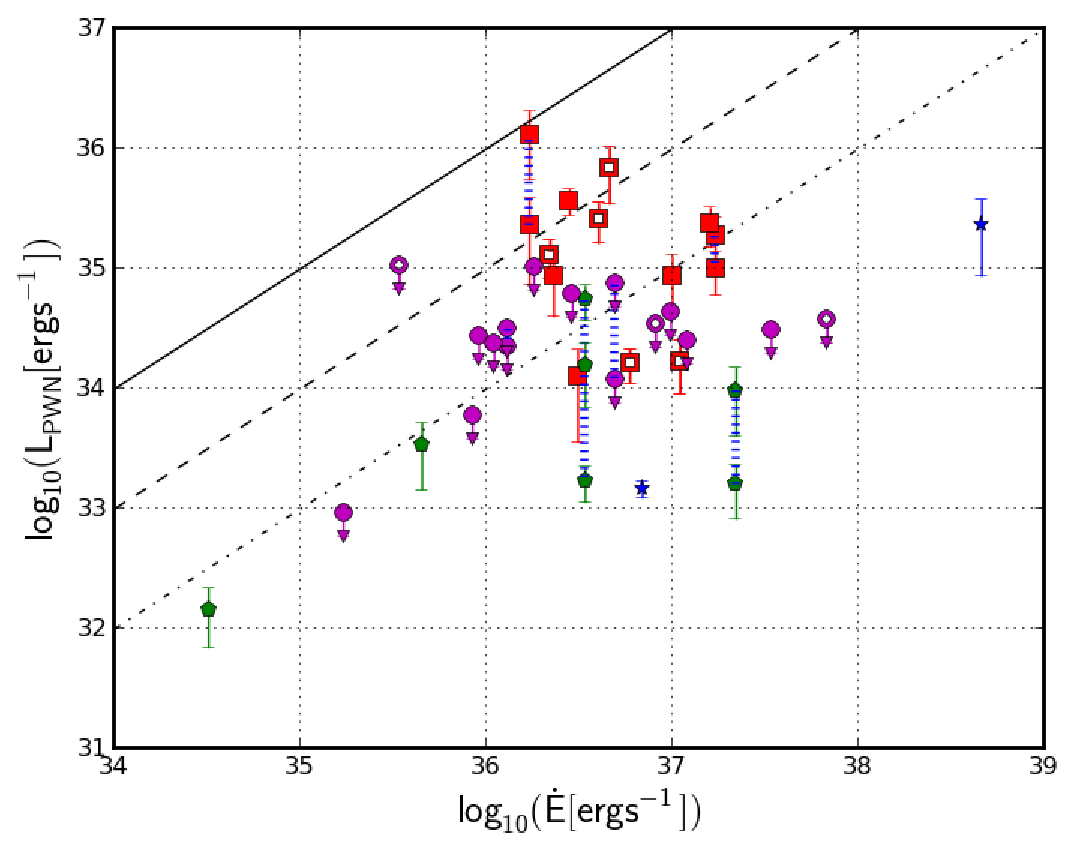
\includegraphics[]{figures/dotelpwn.eps}
\caption{Luminosity of the PWN as a function of the pulsar spin-down power. Full markers correspond to sources with a clear PWN association at TeV energies while hollow markers correspond to sources for which the association between the TeV emission and a PWN is less clear. The red squares (\protect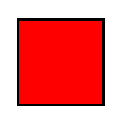
\includegraphics[scale=0.25]{figures/carrerouge.eps}) represent the sources detected at GeV energies, the magenta circles (\protect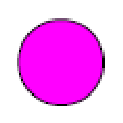
\includegraphics[scale=0.25]{figures/rondmagenta.eps}) show the upper limits, the green pentagon (\protect
\includegraphics[scale=0.25]{figures/pentagonevert.eps}) represent the sources showing a pulsar behaviour in the energy range and the blue stars (\protect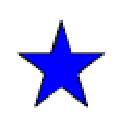
\includegraphics[scale=0.25]{figures/etoilebleue.eps}) represent the Crab nebula and Vela-X not studied in this work. Sources with two distances estimates have two markers connected with a dotted blue line. Pulsars summarized in Table \ref{tab:pulsarfit} are included in the model. 
\label{fig:dotelpwn}}
\end{figure}

\clearpage
